\documentclass[../thesis.tex]{subfiles}

\usepackage{wrapfig}
\usepackage{cite}
% \usepackage{natbib}
% \usepackage[round]{natbib}

\usepackage{amsfonts}       % blackboard math symbols
\usepackage{nicefrac}       % compact symbols for 1/2, etc.
\usepackage{microtype}      % microtypography
\usepackage{amsmath}
\usepackage{tikz}
\usepackage{amsthm}
\usepackage{amssymb}
\usetikzlibrary{positioning}
\usepackage{mathtools}

\newtheorem{theorem}{Theorem}[section]
\newtheorem{assumption}{Assumption}[section]
\newtheorem{proposition}{Proposition}[section]
\newtheorem{definition}{Definition}[section]
\newtheorem{corollary}{Corollary}[theorem]
\newtheorem{lemma}{Lemma}[theorem]
% \newtheorem{corollary}{Corollary}[proposition]
\newtheorem{definition1}{Definition}[section]



% %% editing comment
\newcommand{\cmt}[1]{{\footnotesize\textcolor{red}{#1}}}
\newcommand{\cmto}[1]{{\footnotesize\textcolor{orange}{#1}}}
\newcommand{\note}[1]{\cmt{Note: #1}}
\newcommand{\todo}[1]{\cmt{TO-DO: #1}}
\newcommand{\question}[1]{\cmto{Question: #1}}
\newcommand{\sergey}[1]{{\footnotesize\textcolor{blue}{Sergey: #1}}}
\newcommand{\ak}[1]{{\textcolor{red}{#1}}}
\newcommand{\edits}[1]{\textcolor{red}{#1}}

%% abbreviations
\newcommand{\x}{\mathbf{x}}
\newcommand{\z}{\mathbf{z}}
\newcommand{\y}{\mathbf{y}}
\newcommand{\w}{\mathbf{w}}
\newcommand{\data}{\mathcal{D}}

\newcommand{\etal}{{et~al.}\ }
\newcommand{\eg}{e.g.\ }
\newcommand{\ie}{i.e.\ }
\newcommand{\nth}{\text{th}}
\newcommand{\pr}{^\prime}
\newcommand{\tr}{^\mathrm{T}}
\newcommand{\inv}{^{-1}}
\newcommand{\pinv}{^{\dagger}}
\newcommand{\real}{\mathbb{R}}
\newcommand{\gauss}{\mathcal{N}}
\newcommand{\norm}[1]{\left|#1\right|}
\newcommand{\trace}{\text{tr}}

%% specifics for the paper
\newcommand{\reward}{r}
\newcommand{\policy}{\pi}
\newcommand{\mdp}{\mathcal{M}}
\newcommand{\states}{\mathcal{S}}
\newcommand{\actions}{\mathcal{A}}
\newcommand{\observations}{\mathcal{O}}
\newcommand{\transitions}{T}
\newcommand{\initstate}{d_0}
\newcommand{\freq}{d}
\newcommand{\obsfunc}{E}
\newcommand{\initial}{\mathcal{I}}
\newcommand{\horizon}{H}
\newcommand{\rewardevent}{R}
\newcommand{\probr}{p_\rewardevent}
\newcommand{\metareward}{\bar{\reward}}
\newcommand{\discount}{\gamma}
\newcommand{\behavior}{{\pi_\beta}}
\newcommand{\bellman}{\mathcal{B}}
\newcommand{\qparams}{\phi}
\newcommand{\qparamset}{\Phi}
\newcommand{\qset}{\mathcal{Q}}
\newcommand{\batch}{B}
\newcommand{\qfeat}{\mathbf{f}}
\newcommand{\Qfeat}{\mathbf{F}}
\newcommand{\hatbehavior}{\hat{\pi}_\beta}

\newcommand{\traj}{\tau}

\newcommand{\pihi}{\pi^{\text{hi}}}
\newcommand{\pilo}{\pi^{\text{lo}}}
\newcommand{\ah}{\mathbf{w}}

\newcommand{\proj}{\Pi}

\newcommand{\loss}{\mathcal{L}}
\newcommand{\eye}{\mathbf{I}}

\newcommand{\model}{\hat{p}}

\newcommand{\pimix}{\pi_{\text{mix}}}

\newcommand{\pib}{\bar{\pi}}
\newcommand{\epspi}{\epsilon_{\pi}}
\newcommand{\epsmodel}{\epsilon_{m}}

\newcommand{\return}{\mathcal{R}}

%% math
\newcommand{\cY}{\mathcal{Y}}
\newcommand{\cX}{\mathcal{X}}
\newcommand{\en}{\mathcal{E}}
\newcommand{\be}{\mathbf{e}}
\newcommand{\by}{\mathbf{y}}
\newcommand{\bx}{\mathbf{x}}
\newcommand{\bz}{\mathbf{z}}
\newcommand{\bo}{\mathbf{o}}
\newcommand{\bs}{\mathbf{s}}
\newcommand{\ba}{\mathbf{a}}
\newcommand{\bM}{\mathbf{M}}
\newcommand{\ot}{\bo_t}
\newcommand{\st}{\bs_t}
\newcommand{\at}{\ba_t}
\newcommand{\op}{\mathcal{O}}
\newcommand{\opt}{\op_t}
\newcommand{\kl}{D_\text{KL}}
\newcommand{\tv}{D_\text{TV}}
\newcommand{\ent}{\mathcal{H}}

\newcommand{\bzhi}{\bz^\text{hi}}

\newcommand{\E}{\mathbb{E}}

\newenvironment{repeatedthm}[1]{\@begintheorem{#1}{\unskip}}{\@endtheorem}

% \DeclareMathOperator\supp{supp}



\begin{document}


\blfootnote{This chapter is based on \cite{nakamoto2022calql}, published at NeurIPS 2020, which is joint work with Aurick Zhou, George Tucker, and Sergey Levine.}

A compelling use case of offline reinforcement learning (RL) is to obtain a policy initialization from existing datasets followed by fast online fine-tuning with limited interaction. However, existing offline RL methods tend to behave poorly during fine-tuning. In this paper, we study the fine-tuning problem in the context of conservative offline RL methods and we devise an approach for learning an effective initialization from offline data that also enables fast online fine-tuning capabilities. Our approach, calibrated Q-learning (\methodname), accomplishes this by learning a conservative value function initialization that underestimates the value of the learned policy from offline data, while also ensuring that the learned Q-values are at a reasonable scale. We refer to this property as calibration, and define it formally as providing a lower bound on the true value function of the learned policy and an upper bound on the value of some other (suboptimal) reference policy, which may simply be the behavior policy. We show that a conservative offline RL algorithm that also learns a calibrated value function leads to effective online fine-tuning, enabling us to take the benefits of offline initializations in online fine-tuning. In practice, \methodname\ can be implemented on top of the conservative Q learning (CQL)~\cite{kumar2020conservative} for offline RL within a one-line code change. Empirically, \methodname\ outperforms state-of-the-art methods on {\bf 9/11} fine-tuning benchmark tasks that we study in this paper.     

\vspace{-0.2cm}
\section{Introduction}
\label{sec:calql_introduction}
\vspace{-0.2cm}

Modern machine learning successes follow a common recipe: pre-training models on general-purpose, Internet-scale data, followed by fine-tuning the pre-trained initialization on a limited amount of data for the task of interest~\cite{he2022masked,devlin2018bert}. How can we translate such a recipe to sequential decision-making problems? A natural way to instantiate this paradigm is to utilize offline RL for initializing value functions and policies from static datasets, followed by online fine-tuning to improve this initialization with limited active interaction. If successful, such a recipe might enable effective online RL with much fewer samples than current methods that learn from scratch.

Many algorithms for offline RL have been applied to online fine-tuning. Empirical results across such works suggest a counter-intuitive trend: policy initializations obtained from more effective offline RL methods tend to exhibit worse online fine-tuning performance, even within the same task (see Table 2 of~\cite{kostrikov2021offline} \& Figure 4 of \cite{xiao2023the}). On the other end, online RL methods training from scratch (or RL from demonstrations~\cite{vecerik2017leveraging},
where the replay buffer is seeded with the offline data) seem to improve online at a significantly faster rate. But these online methods require actively collecting data by rolling out policies from scratch, which inherits similar limitations to na\"ive online RL methods in problems where data collection is expensive or dangerous. Overall, these results suggest that it is challenging to devise an offline RL algorithm that both acquires a good initialization from prior data and also enables efficient fine-tuning.

\begin{wrapfigure}{r}{0.5\columnwidth}
    % \vspace{-1.6cm}
    \vspace{-0.3cm}
    \begin{center}
    {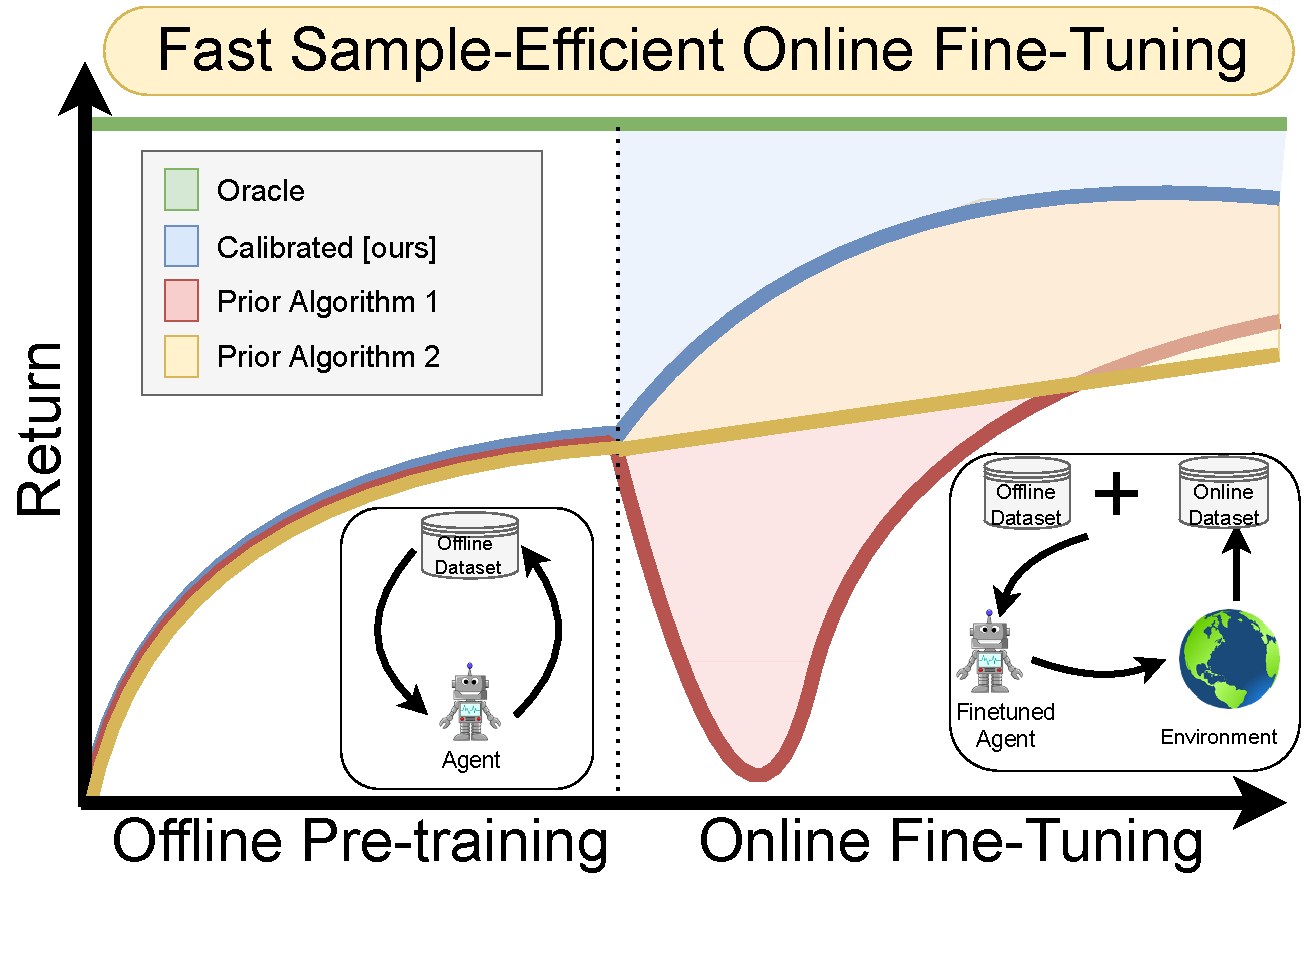
\includegraphics[width=0.85\linewidth]{chapters/cal_ql/figs-sample/Teaser_V2.pdf}}
    \vspace{-0.4cm}
    \caption{
    \footnotesize{We study \textbf{offline RL pre-training followed by online RL fine-tuning}. Some prior offline RL methods tend to exhibit slow performance improvement in this setting (yellow), resulting in worse asymptotic performance. Others suffer from initial performance degradation once online fine-tuning begins (red), resulting in a high cumulative regret. We develop an approach that ``\emph{calibrates}'' the value function to attain a fast improvement with a smaller regret (blue).}}
    \vspace{-0.7cm}
    \label{fig:teaser}
    \end{center}
\end{wrapfigure}
How can we devise a method to learn an effective policy initialization that also improves during fine-tuning? We have shown that one can learn a good offline initialization by optimizing the policy against a \emph{conservative} value function obtained from an offline dataset. But, as we show in Section~\ref{sec:calql_empirical_analysis}, conservatism alone is insufficient for efficient online fine-tuning. Conservative methods often tend to ``unlearn'' the policy initialization learned from offline data and waste samples collected via online interaction in recovering this initialization. We find that the ``unlearning'' phenomenon is a consequence of the fact that value estimates produced via conservative methods can be significantly lower than the ground-truth return of \emph{any} valid policy. Having Q-value estimates that do not lie on a similar scale as the return of a valid policy is problematic. Because once fine-tuning begins, actions executed in the environment for exploration that are actually worse than the policy learned from offline data could erroneously appear better, if their ground-truth return value is larger than the learned conservative value estimate. Hence, subsequent policy optimization will degrade the policy performance until the method recovers.  

% Our approach
If we can ensure that the conservative value estimates learned using the offline data are \emph{calibrated}, meaning that these estimates are on a similar scale as the true return values, then we can avoid the unlearning phenomenon caused by conservative methods (see the formal definition in~\ref{cond:calibration}). Of course, we cannot enforce such a condition perfectly, since it would require eliminating all errors in the value function. Instead, we devise a method for ensuring that the learned values upper bound the true values of some \emph{reference policy} whose values can be estimated more easily (e.g., the behavior policy), while still lower bounding the values of the learned policy. Though this does not perfectly ensure that the learned values are correct, we show that it still leads to sample-efficient online fine-tuning. Thus, our practical method, \textbf{calibrated Q-learning} \textbf{(\methodname)}, learns conservative value functions that are ``calibrated'' against the behavior policy, via a simple modification to existing conservative methods.

The main contribution of this chapter is \methodname, a method for acquiring an offline initialization that facilitates online fine-tuning. \methodname\ aims to learn conservative value functions that are calibrated with respect to a reference policy (e.g., the behavior policy). Our analysis of \methodname\ shows that \methodname\ attains stronger guarantees on cumulative regret during fine-tuning. In practice, \methodname\ can be implemented on top of conservative Q-learning~\cite{kumar2020conservative}, a prior offline RL method, without any additional hyperparameters. We evaluate \methodname\ across a range of benchmark tasks from \cite{fu2020d4rl}, \cite{singh2020cog} and \cite{AWAC}, including robotic manipulation and navigation. We show that \methodname\ matches or outperforms the best methods on all tasks, in some cases by 30-40\%.


\vspace{-0.2cm}
\section{Related Work}
\vspace{-0.3cm}
Several prior works suggest that online RL methods typically require a large number of samples~\cite{silver2016mastering,vinyals2019grandmaster,ye2020towards,kakade2002approximately,zhai2022computational,gupta2022unpacking,li2022understanding} to learn from scratch. We can utilize offline data to accelerate online RL algorithms. Prior works do this in a variety of ways: incorporating the offline data into the replay buffer of online RL~\cite{schaal1996learning,vecerik2017leveraging,hester2018deep,song2023hybrid}, utilizing auxiliary behavioral cloning losses with policy gradients~\cite{rajeswaran2017learning,kang2018policy,zhu2018reinforcement,zhu2019dexterous}, or extracting a high-level skill space for downstream online RL~\cite{gupta2019relay,ajay2020opal}. While these methods improve the sample efficiency of online RL from scratch, as we will also show in our results, they do not eliminate the need to actively roll out poor policies for data collection.

To address this issue, a different line of work first runs offline RL for learning a good policy and value initialization from the offline data, followed by online fine-tuning~\cite{nair2020accelerating,kostrikov2021iql,lyu2022mildly,beeson2022improving,wu2022supported,lee2022offline,mark2022fine}. These approaches typically employ offline RL methods based on policy constraints or pessimism~\cite{fujimoto2018off,siegel2020keep,guo2020batch,ghasemipour2021emaq,kostrikov2021iql,singh2020cog,lee2022offline} on the offline data, then continue training with the same method on a combination of offline and online data once fine-tuning begins~\cite{nachum2019algaedice,kidambi2020morel,yu2020mopo,kumar2020conservative,buckman2020importance}. Although pessimism is crucial for offline RL~\cite{jin2021pessimism,cheng2022adversarially}, using pessimism or constraints for fine-tuning~\cite{nair2020accelerating,kostrikov2021iql,lyu2022mildly} slows down fine-tuning or leads to initial unlearning, as we will show in Section~\ref{sec:calql_empirical_analysis}. In effect, these prior methods either fail to improve as fast as online RL or lose the initialization from offline RL. We aim to address this limitation by understanding some conditions on the offline initialization that enable fast fine-tuning. 

Our approach is most related to methods that utilize a pessimistic offline RL algorithm for offline training but incorporate exploration in fine-tuning~\cite{lee2022offline,mark2022fine,wu2022supported}. In contrast to these works, our method aims to learn a better offline initialization that enables standard online fine-tuning. Our approach fine-tunes na\"ively without ensembles~\cite{lee2022offline} or exploration~\cite{mark2022fine} and, as we show in our experiments, this alone is enough to outperform approaches that employ explicit optimism during data collection.
\vspace{-0.2cm}
\section{Problem Statement and Additional Notation}
\vspace{-0.2cm}
% The goal in RL is to learn the optimal policy for an MDP $\mathcal{M} = (\mathcal{S}, \mathcal{A}, P, r, \rho, \gamma)$. $\mathcal{S}, \mathcal{A}$ denote the state and action spaces.  $P(s' | s, a)$ and $r(s,a)$
% are the dynamics and reward functions. $\rho(s)$ denotes the initial state distribution.  $\gamma \in (0,1)$ denotes the discount factor. Formally, the goal is to learn a policy $\pi:\mc S\mapsto \mc A$ that maximizes cumulative discounted value function, denoted by $V^\pi(s) = {\frac{1}{1-\gamma}\sum_{t} \bb E_{a_t \sim \pi(s_t)}\brac{\gamma^t r(s_t, a_t)|s_0=s}}$. The Q-function of a given policy $\pi$ is defined as ${Q^\pi(s,a) = {\frac{1}{1-\gamma}\sum_{t} \bb E_{a_t \sim \pi(s_t)}\brac{\gamma^t r(s_t, a_t)|s_0=s,a_0=a}}}$, and we use $Q_\theta^\pi$ to denote the estimate of the Q-function of a policy $\pi$ as obtained via a neural network with parameters $\theta$.

Given access to an offline dataset $\mathcal{D} = \{(s, a, r, s^\prime)\}$ collected using a behavior policy $\behavior$, we aim to first train a good policy and value function using the offline dataset $\mathcal{D}$ alone, followed by an online phase that utilizes online interaction in $\mathcal{M}$. Our goal during fine-tuning is to obtain the optimal policy with the smallest number of online samples. This can be expressed as minimizing the \textbf{cumulative regret} over rounds of online interaction: 
\begin{align}
\regret(K) := \bb E_{s\sim \rho}\sum_{k=1}^K\brac{V^{\star}(s) - V^{\pi^k}(s)}. 
\end{align}
% As we demonstrate in Section~\ref{sec:experiments}, existing methods face challenges in this setting.

% Our approach will build on the conservative Q-learning (CQL)~\cite{kumar2020conservative} algorithm.
% CQL imposes an additional regularizer that penalizes the learned Q-function on out-of-distribution (OOD) actions while compensating for this pessimism on actions seen within the training dataset. Assuming that the value function is represented by a function, $Q_\theta$, the training objective of CQL is given by
% \begin{align}
%     \label{eqn:cql_training}
%     \!\!\!\!\!\min_\theta {\color[HTML]{6C8EBF} {\alpha \underbrace{\left(\mathbb{E}_{s \sim \mathcal{D}, a \sim \pi} \left[Q_\theta(s,a)\right] - \mathbb{E}_{s, a \sim \mathcal{D}}\left[Q_\theta(s,a)\right]\right)}_{\text{Conservative regularizer }\mathcal{R}(\theta)}}} + \frac{1}{2} {\mathbb{E}_{s, a, s^\prime\sim \mathcal{D}}\left[\left(Q_\theta(s, a) - \bellman^\pi\bar{Q}(s, a)\right)^2 \right]},
% \end{align}
% where $\bellman^\pi \bar{Q} (s, a)$ is the backup operator applied to a delayed target Q-network, $\bar{Q}$: $\bellman^\policy \bar{Q}(s, a) := r(s, a) + \gamma \E_{a^\prime \sim \pi(a^\prime|s^\prime)}[\bar{Q}(s^\prime, a^\prime)]$. The second term is the standard TD error~\cite{lillicrap2015continuous,fujimoto2018addressing,haarnoja2018sacapps}. The first term  $\mathcal{R}(\theta)$ (in {\color[HTML]{6C8EBF} blue}) is a conservative regularizer that aims to prevent overestimation in the Q-values for OOD actions by minimizing the Q-values under the policy $\pi(\ba|\bs)$, and counterbalances by maximizing the Q-values of the actions in the dataset following the behavior policy $\pi_\beta$.

% \vspace{-0.2cm}
\vspace{-0.2cm}
\section{When Can Offline RL Initializations Enable Fast Online Fine-Tuning?}
\label{sec:empirical}
\vspace{-0.2cm}

A starting point for offline pre-training and online fine-tuning is to simply initialize the value function with one that is produced by an existing offline RL method and then perform fine-tuning. However, we empirically find that initializations learned by many offline RL algorithms can perform poorly during fine-tuning. We will study the reasons for this poor performance for the subset of conservative methods to motivate and develop our approach for online fine-tuning, calibrated Q-learning. 

\vspace{-0.1cm}
\subsection{Empirical Analysis}
\label{sec:empirical_analysis}
\vspace{-0.2cm}

\begin{wrapfigure}{r}{0.38\columnwidth}
\vspace{-1.0cm}
\begin{center}
{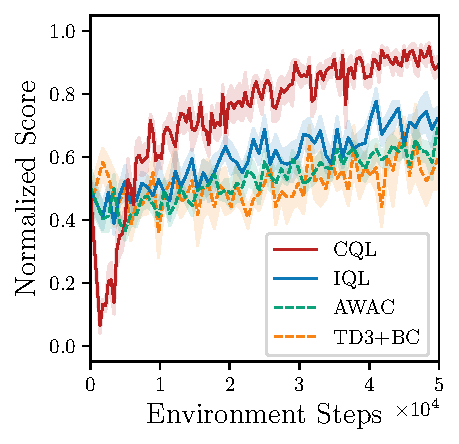
\includegraphics[width=0.78\linewidth]{chapters/cal_ql/figs-sample/sec41-final-utd5.pdf}}
\vspace{-0.3cm}
\caption{\label{fig:cql_iql_finetune}\footnotesize{\textbf{Multiple prior offline RL algorithms suffer from difficulties} during fine-tuning including poor asymptotic performance and initial unlearning.}}
\vspace{-0.7cm}
\end{center}
\end{wrapfigure}
Offline RL followed by online fine-tuning typically poses non-trivial challenges for a variety of methods. While analysis in prior work~\citep{nair2020accelerating} notes challenges for a subset of offline RL methods, in Figure~\ref{fig:cql_iql_finetune}, we evaluate the fine-tuning performance of a variety of prior offline RL methods (CQL~\citep{kumar2020conservative}, IQL~\citep{kostrikov2021offlineb}, TD3+BC~\citep{fujimoto2021minimalist}, AWAC~\citep{nair2020accelerating}) on a particular diagnostic instance of a visual pick-and-place task with a distractor object and sparse binary rewards~\citep{singh2020cog}, and find that all methods struggle to attain the best possible performance, quickly. More details about this task are in Appendix~\ref{appendix:env_details}. 

% The analysis by \citet{nair2020accelerating} highlights the limitations of explicit policy constraint methods for fine-tuning. Therefore, in this section, we study a representative \emph{implicit} policy constraint method, implicit Q-learning (IQL)~\cite{kostrikov2021offlineb} that attains good performance on benchmark tasks, and a conservative method, CQL~\cite{kumar2020conservative}.
%%SL.5.7: I really think we should just remove the IQL discussion here. We don't actually "study" IQL in any meaningful way here, and the reference to Nair et al. is pretty tortured too. We could just say we'll use CQL as our starting point, though the issues we observe have also been noted with other RL methods (and we can reference Nair for that, since the AWAC paper also observes the "dip").
%%SZ.5.9: agree
% We study the task of fine-tuning a robot policy on a visual pick-and-place task with a distractor object and sparse binary rewards, from prior work~\cite{singh2020cog}. 
% More details about the offline dataset are in Appendix~\ref{appendix:env_details}.  

% We present the learning curves for both methods in online fine-tuning in Figure~\ref{fig:cql_iql_finetune}. 
While the offline Q-function initialization obtained from all methods attains a similar (normalized) return of around 0.5, they suffer from difficulties during fine-tuning: TD3+BC, IQL, AWAC attain slow asymptotic performance and CQL unlearns the offline initialization, followed by spending a large amount of online interaction to recover the offline performance again, before any further improvement. This initial unlearning appears in multiple tasks as we show in Appendix~\ref{app:cql_dip_zoom_in}. In this work, we focus on developing effective fine-tuning strategies on top of conservative value estimation methods like CQL. To do so, we next aim to understand the potential reason behind the initial unlearning in CQL.  

\begin{wrapfigure}{r}{0.6\linewidth}
\vspace{-0.5cm}
\begin{center}
\centerline{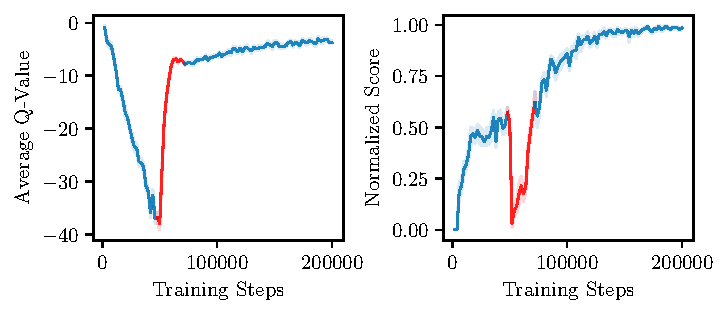
\includegraphics[width=0.99\linewidth]{chapters/cal_ql/figs-sample/CQL-q-values.pdf}}
\vspace{-0.25cm}
\caption{\label{fig:cql_q_value} \footnotesize{\textbf{The evolution of the average Q-value and the success rate of CQL over the course of offline pre-training and online fine-tuning.} Fine-tuning begins at 50K steps. The red-colored part denotes the period of performance recovery which also coincides with the period of Q-value adjustment.}}
\end{center}
\vspace{-0.9cm}
\end{wrapfigure}
\textbf{Why does CQL unlearn initially?} To understand why CQL unlearns initially, we inspect the learned Q-values averaged over the dataset in Figure~\ref{fig:cql_q_value}. Observe that the Q-values learned by CQL in the offline phase are \emph{much} smaller than their ground-truth value (as expected), but these Q-values drastically jump and adjust in scale when fine-tuning begins. In fact, we observe that performance recovery (red segment in Figure~\ref{fig:cql_q_value}) {\em coincides} with a period where the range of Q-values changes to match the true range. This is as expected: as a conservative Q-function experiences new online data, actions much worse than the offline policy on the rollout states appear to attain higher rewards compared to the highly underestimated offline Q-function, which in turn deceives the policy optimizer into unlearning the initial policy. We illustrate this idea visually in Figure~\ref{fig:calql_idea}. Once the Q-function has adjusted and the range of Q-values closely matches the true range, then fine-tuning can proceed normally, after the dip. 


\textbf{To summarize,} our empirical analysis indicates that methods existing fine-tuning methods suffer from difficulties such as initial unlearning or poor asymptotic performance. In particular, we observed that conservative methods can attain good asymptotic performance, but ``waste'' samples to correct the learned Q-function. Thus, in this paper, we attempt to develop a good fine-tuning method that builds on top of an existing conservative offline RL method, CQL, but aims to ``calibrate'' the Q-function so that the initial dip in performance can be avoided. 

\vspace{-0.1cm}
\subsection{Conditions on the Offline Initialization that Enable Fast Fine-Tuning}
\vspace{-0.18cm}
Our observations from the preceding discussion motivate two conclusions in regard to the offline Q-initialization for fast fine-tuning: \textbf{(a)} methods that learn \textbf{conservative} Q-functions can attain good asymptotic performance, and \textbf{(b)} if the learned Q-values closely match the range of ground-truth Q-values on the task, then online fine-tuning does not need to devote samples to unlearn and then recover the offline initialization. One approach to formalize this intuition of Q-values lying on a similar scale as the ground-truth Q-function is via the requirement that the conservative Q-values learned by the conservative value estimation method must be lower-bounded by the ground-truth Q-value of a sub-optimal reference policy. This will prevent conservatism from learning overly small Q-values. We will refer to this property as ``calibration'' with respect to the reference policy.
\begin{tcolorbox}[colback=blue!6!white,colframe=black,boxsep=0pt,top=-3pt,bottom=2pt]
\vspace{2mm}
\begin{definition}[Calibration]
\label{cond:calibration}
An estimated Q-function ${Q}_\theta^\pi$ for a given policy $\pi$ is said to be calibrated with respect to a reference policy $\mu$ if:
\begin{align} 
    \mathbb{E}_{\mathbf{a} \sim \pi}\left[Q_\theta^\pi(\bs, \mathbf{a})\right] \geq \mathbb{E}_{\mathbf{a} \sim \mu}\left[Q^\mu(\bs, \mathbf{a})\right] := V^\mu(s), \forall s \in \mc \mathcal{D}.
\end{align}
\end{definition}
\end{tcolorbox}

If the learned Q-function ${Q}^\pi_\theta$ is calibrated with respect to a policy $\mu$ that is worse than $\pi$, it would prevent unlearning during fine-tuning that we observed in the case of CQL.
This is because the policy optimizer would not unlearn $\pi$ in favor of a policy that is worse than the reference policy $\mu$ upon observing new online data as the expected value of $\pi$ is constrained to be larger than $V^\mu$: $\mathbb{E}_{\mathbf{a} \sim \pi}\left[{Q}^\pi_\theta(\bs, \mathbf{a})\right] \geq V^\mu(\bs)$.
Our practical approach \methodname\ will enforce calibration with respect to a policy $\mu$ whose ground-truth value, $V^\mu(\bs)$, can be estimated reliably without bootstrapping error (e.g., the behavior policy induced by the dataset). This is the key idea behind our method (as we will discuss next) and is visually illustrated in Figure~\ref{fig:calql_idea}.

\vspace{-0.2cm}
\vspace{-0.1cm}
\section{\methodname: Calibrated Q-Learning}
\label{sec:empirical-method}
\vspace{-0.25cm}
Our approach, calibrated Q-learning (\methodname) aims to learn a conservative and calibrated value function initializations from an offline dataset. To this end, \methodname\ builds on CQL from Chapter ?? and then constrains the learned Q-function to produce Q-values larger than the Q-value of a reference policy $\mu$ per Definition~\ref{cond:calibration}. In principle, our approach can utilize many different choices of reference policies, but for developing a practical method, we simply utilize the behavior policy as our reference policy.  

~

\niparagraph{\textbf{Calibrating CQL.}} We can constrain the learned Q-function $Q^\pi_\theta$ to be larger than $V^\mu$ via a simple change to the CQL training objective (Equation~\ref{eqn:cql_training}): masking out the push down of the learned Q-value on out-of-distribution (OOD) actions in CQL if the Q-function is not calibrated, i.e., if $\mathbb{E}_{a \sim \pi}\left[Q^\pi_\theta(\bs, \mathbf{a})\right] \leq V^\mu(\bs)$. \methodname\ modifies the CQL regularizer, $\mathcal{R}(\theta)$ in this manner: 
\begin{align}
\label{eqn:cal_ql_training}
\!\!\!\!\!\!\mathbb{E}_{\bs \sim \mathcal{D}, \mathbf{a} \sim \pi} \brac{{\color[HTML]{B85450}{\max \left( Q_\theta(s,a), V^\mu(s) \right)}} } - \mathbb{E}_{\bs, \mathbf{a} \sim \mathcal{D}}\left[Q_\theta(\bs,\mathbf{a})\right],
\end{align}
where the changes from standard CQL are depicted in {\color[HTML]{B85450} red}. As long as $\alpha$ (in Equation~\ref{eqn:cql_training}) is large, for any state-action pair where the learned Q-value is smaller than $Q^\mu$, the Q-function in Equation~\ref{eqn:cal_ql_training} will upper bound $Q^\mu$ in a tabular setting. Of course, as with any practical RL method, with function approximators and gradient-based optimizers, we cannot guarantee that we can enforce this condition for every state-action pair, but in our experiments, we find that Equation~\ref{eqn:cal_ql_training} is sufficient to enforce the calibration in expectation over the states in the dataset.         

\begin{wrapfigure}{r}{0.65\linewidth}
\centering
\vspace{-0.2cm}
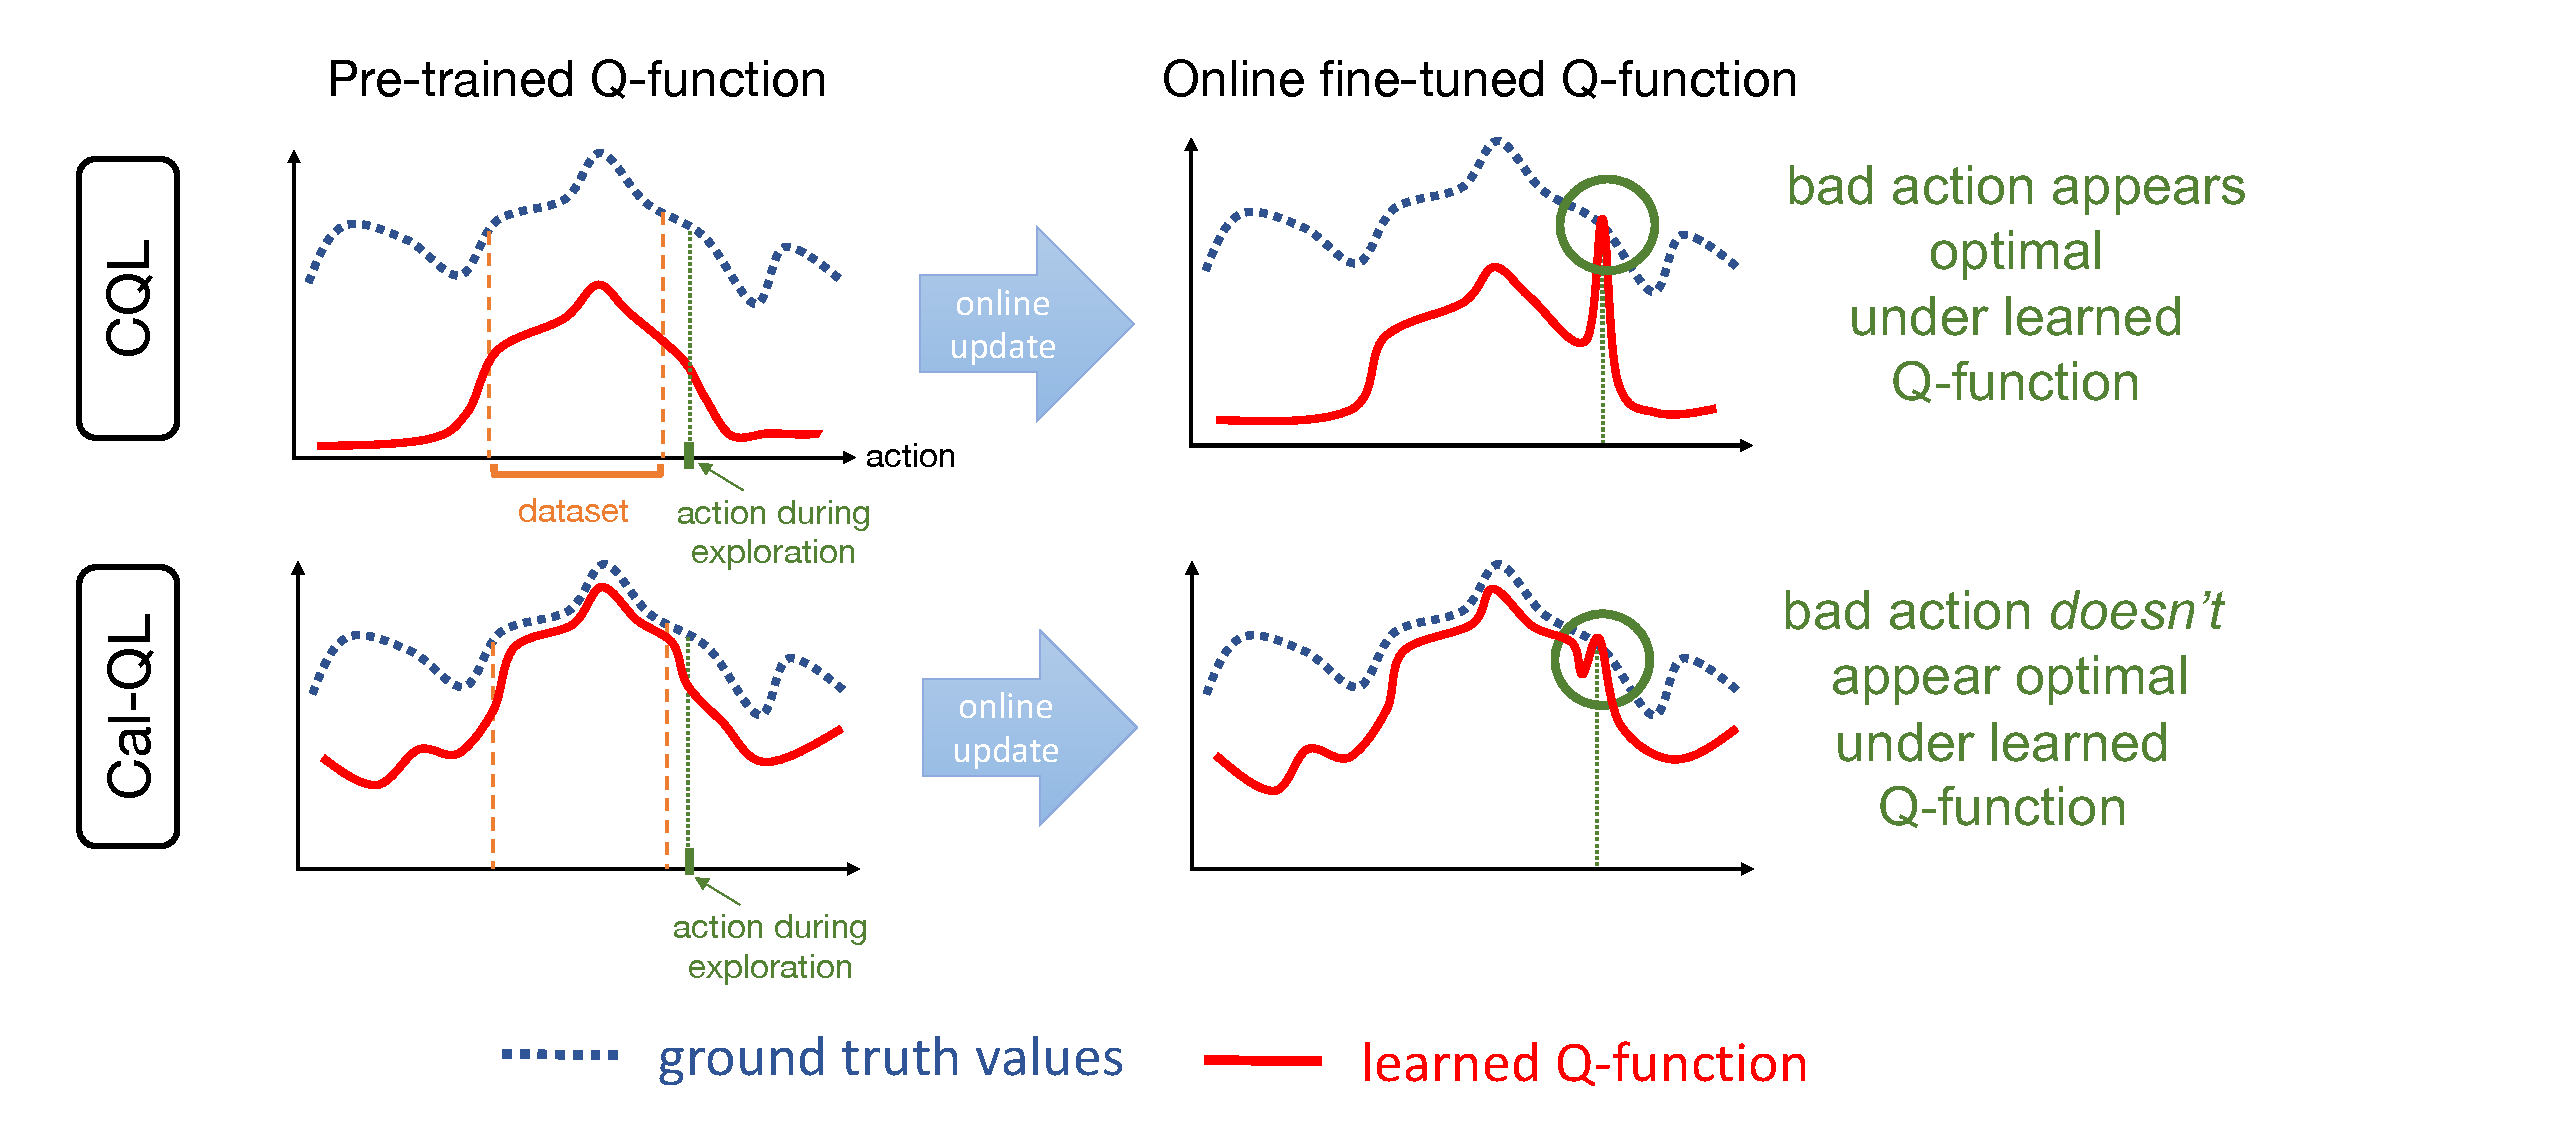
\includegraphics[trim={0 0 2.7cm 0},clip,width=0.98\linewidth]{chapters/cal_ql/figs-sample/figure_for_calql_final.pdf}
\vspace{-0.2cm}
\caption{
\footnotesize{\textbf{Intuition behind policy unlearning with CQL and the idea behind \methodname.} The plot visualizes a slice of the learned Q-function and the ground-truth values for a given state. Erroneous peaks on suboptimal actions (x-axis) arise when updating CQL Q-functions with online data. This in turn can lead the policy to deviate away from high-reward actions covered by the dataset in favor of erroneous new actions, resulting in deterioration of the pre-trained policy. In contrast, \methodname\ corrects the scale of the learned Q-values by using a reference value function, such that actions with worse Q-values than the reference value function do not erroneously appear optimal in fine-tuning.}}
\label{fig:calql_idea}
\vspace{-0.4cm}
\end{wrapfigure}

~

\niparagraph{\textbf{Pseudo-code and implementation details.}} Our implementation of \methodname\ directly builds on the implementation of CQL from \citet{geng2022jaxcql}. We present a pseudo-code for \methodname\ in Algorithm~\ref{alg:practical_alg}. Additionally, we list the hyperparameters $\alpha$ for the CQL algorithm and our baselines for each suite of tasks in Appendix \ref{app:hyperparam}. Following the protocol in prior work~\citep{kostrikov2021offlineb,song2023hybrid}, the practical implementation of \methodname\ trains on a mixture of the offline data and the new online data, weighted in some proportion during fine-tuning. To get $V^\mu(\bs)$, we can fit a function approximator $Q^\mu_\theta$ or $V^\mu_\theta$ to the return-to-go values via regression, but we observed that also simply utilizing the return-to-go estimates for tasks that end in a terminal was sufficient for our use case. We show in  Section~\ref{sec:experiments}, how this simple \emph{one-line} change to the objective drastically improves over prior fine-tuning results.

\vspace{-0.2cm}
\vspace{-0.15cm}
\section{Theoretical Intuition of \methodname}
\label{sec:theory}
\vspace{-0.25cm}

We will now analyze the cumulative regret attained over online fine-tuning, when the value function is pre-trained with Cal-QL, and show that enforcing calibration (Defintion~\ref{cond:calibration}) leads to a favorable regret bound during the online phase. Our analysis utilizes tools from \citet{song2023hybrid}, but studies the impact of calibration on fine-tuning. We also remark that we simplify the treatment of certain aspects (e.g., how to incorporate pessimism) as it allows us to cleanly demonstrate benefits of calibration.  

~

\niparagraph{\textbf{Notation \& terminology.}} In our analysis, we will consider an idealized version of \methodname\ for simplicity. Specifically, following prior work~\citep{song2023hybrid} under the bilinear model~\citep{du2021bilinear}, we will operate in a finite-horizon setting with a horizon $H$. We denote the learned Q-function at each learning iteration $k$ for a given $(\bs, \mathbf{a})$ pair and time-step $h$ by $Q_{\theta}^k(\bs, \mathbf{a})$. For any given policy $\pi$, let $C_\pi\geq1$ denote the concentrability coefficient such that $C_\pi:=\max_{f\in \mc C}\frac{\sum_{h=0}^{H-1}\bb E_{s,a\sim d_h^\pi}[\mc T f_{h+1}(s,a)-f_h(s,a)]}{\sqrt{\sum_{h=0}^{H-1}\bb E_{s,a\sim \nu_h}(\mc T f_{h+1}(s,a)-f_h(s,a))^2}}$,
i.e., a coefficient that quantifies the distribution shift between the policy $\pi$ and the dataset $\mathcal{D}$, in terms of the ratio of Bellman errors averaged under $\pi$ and the dataset $\mathcal{D}$. Note that $\mc C$ represents the Q-function class and we assume $\mc C$ has a bellman-bilinear rank~\citep{du2021bilinear} of $d$. We also use $C_\pi^\mu$ to denote the concentrability coefficient over a subset of {\em calibrated} Q-functions w.r.t. a reference policy $\mu$: $C^\mu_\pi:=\max_{f\in \mc C,f(s,a)\geq Q^\mu(s,a)}\frac{\sum_{h=0}^{H-1}\bb E_{s,a\sim d_h^\pi}[\mc T f_{h+1}(s,a)-f_h(s,a)]}{\sqrt{\sum_{h=0}^{H-1}\bb E_{s,a\sim \nu_h}(\mc T f_{h+1}(s,a)-f_h(s,a))^2}}$, which provides $C^\mu_\pi\leq C_\pi$. Similar to $\mc C$, let $d_\mu$ denote the bellman bilinear rank of $\mc C_\mu$ -- 
the calibrated Q-function class w.r.t. the reference policy $\mu$.
Intuitively, we have $\mc C_\mu\subset\mc C$, which implies that $d_\mu\leq d$. The formal definitions are provided in Appendix~\ref{appendix:notations}.
We will use $\pi^k$ to denote the arg-max policy induced by $Q^k_\theta$. 

% \vspace{-0.4cm}
% \subsection{Intuition} 
% \vspace{-0.4cm}

~

\niparagraph{\textbf{Intuition.}} We intuitively discuss how calibration and conservatism enable \methodname\ to attain a smaller regret compared to not imposing calibration. Our goal is to bound the cumulative regret of online fine-tuning, ${\sum_{k} \mathbb{E}_{\bs_0 \sim \rho}[V^{\pi^\star}(\bs_0) - V^{\pi^k}(\bs_0)]}$. We can decompose this expression into two terms: 
\vspace{-0.05cm}
\begin{align}
    \resizebox{.87\textwidth}{!}{$\regret(K) = \underbrace{\sum_{k=1}^K \mathbb{E}_{\bs_0 \sim \rho} \brac{V^{\star}(\bs_0) -\max_a {Q}_{\theta}^k(\bs_0,\mathbf{a})}}_{(i) ~:=~ \text{miscalibration}}
    +\underbrace{\sum_{k=1}^K \mathbb{E}_{\bs_0 \sim \rho} \brac{ \max_a {Q}_{\theta}^k(\bs_0,\mathbf{a}) - V^{\pi^{k}}(\bs_0)}}_{(ii) ~:=~ \text{overestimation}}$.}
\label{eq:regret-decomposition}
\end{align}
This decomposition of regret into terms (i) and (ii) is instructive. Term (ii) corresponds to the amount of over-estimation in the learned value function, which is expected to be small if a conservative RL algorithm is used for training. Term (i) is the difference between the ground-truth value of the optimal policy and the learned Q-function and is negative if the learned Q-function were calibrated against the optimal policy (per Definition~\ref{cond:calibration}). Of course, this is not always possible because we do not know $V^\star$ a priori. But note that when \methodname\ utilizes a reference policy $\mu$ with a high value $V^\mu$, close to $V^\star$, then the learned Q-function $Q_\theta$ is calibrated with respect to $Q^\mu$ per Condition~\ref{cond:calibration} and term (i) can still be controlled. Therefore, controlling this regret requires striking a balance between learning a calibrated (term (i)) and conservative (term (ii)) Q-function. We now formalize this intuition and defer the detailed proof to Appendix~\ref{appdendix:derivation-CalQL}. 

% \vspace{-0.2cm}
% \subsection{Theorem Statement}
% \vspace{-0.15cm}

% \iffalse

\begin{tcolorbox}[colback=blue!6!white,colframe=black,boxsep=0pt,top=-3pt,bottom=2pt]
\vspace{2mm}
\begin{theorem}[Informal regret bound of \methodname]
\label{thm:main-thm-informal}
    With high probability, \methodname{} obtains the following bound on total regret accumulated during online fine-tuning: \vspace{-0.15cm}
\begin{equation*}
    \begin{split}
        \regret(K) = \wt{O}\Big(\min\big\{C_{\pi^\star}^\mu H\sqrt{dK\log\paren{|\mc F|}},
        \;K\mathbb{E}_{\rho}[V^{\star}(\bs_0) -V^\mu(\bs_0)]+H\sqrt{d_\mu K\log\paren{|\mc F|}}\big\}\Big),
    \end{split}
\end{equation*}
where $\mc F$ is the functional class of the Q-function.
\end{theorem}
\end{tcolorbox}

\niparagraph{\textbf{Comparison to~\citet{song2023hybrid}.}}
\citet{song2023hybrid} analyzes an online RL algorithm that utilizes offline data without imposing conservatism or calibration. We now compare Theorem~\ref{thm:main-thm-informal} to Theorem 1 of \citet{song2023hybrid} to understand the impact of these conditions on the final regret guarantee. Theorem 1 of \citet{song2023hybrid} presents a regret bound: $\regret(K) = \wt{O}\left( C_{\pi^\star} H \sqrt{d K \log\paren{|\mc F|}} \right)$ and we note some improvements in our guarantee, that we also verify via experiments in Section~\ref{subsec:diagonistic}: \textbf{(a)} for the setting where the reference policy $\mu$ contains near-optimal behavior, i.e., $V^\star - V^\mu \lesssim O(H\sqrt{d\log\paren{|\mc F|}/K})$, \methodname\ can enable a tighter regret guarantee compared to \citet{song2023hybrid}; \textbf{(b)} as we show in Appendix~\ref{subsec:CalQL-assumptions}, the concentrability coefficient $C^\mu_{\pi^\star}$ appearing in our guarantee is no larger than the one that appears in Theorem 1 of \citet{song2023hybrid}, providing another source of improvement; and \textbf{(c)} finally, in the case where the reference policy has broad coverage \emph{and} is highly sub-optimal, \methodname\ reverts back to the guarantee from \citep{song2023hybrid}, meaning that \methodname\ improves upon this prior work.

% \fi


\vspace{-0.2cm}
\vspace{-0.09cm}
\section{Experimental Evaluation}
\vspace{-0.22cm}
\label{sec:experiments}
The goal of our experimental evaluation is to study how well \methodname\ can facilitate sample-efficient online fine-tuning. To this end, we compare \methodname\ with several other state-of-the-art fine-tuning methods on a variety of offline RL benchmark tasks from D4RL~\cite{fu2020d4rl}, \citet{singh2020cog}, and \citet{nair2020accelerating}, evaluating performance before and after fine-tuning. We also study the effectiveness of \methodname\ on higher-dimensional tasks, where the policy and value function must process raw image observations. Finally, we perform empirical studies to understand the efficacy of \methodname\ with different dataset compositions and the impact of errors in the reference value function estimation.
% to understand the efficacy of \methodname\ with different dataset compositions 
% Finally, we perform several empirical studies to understand the efficacy of \methodname\ with different dataset compositions and to understand the impact of errors in reference function value estimation on \methodname.  

~

\begin{wrapfigure}{r}{0.48\linewidth}
\centering
\vspace{-0.45cm}
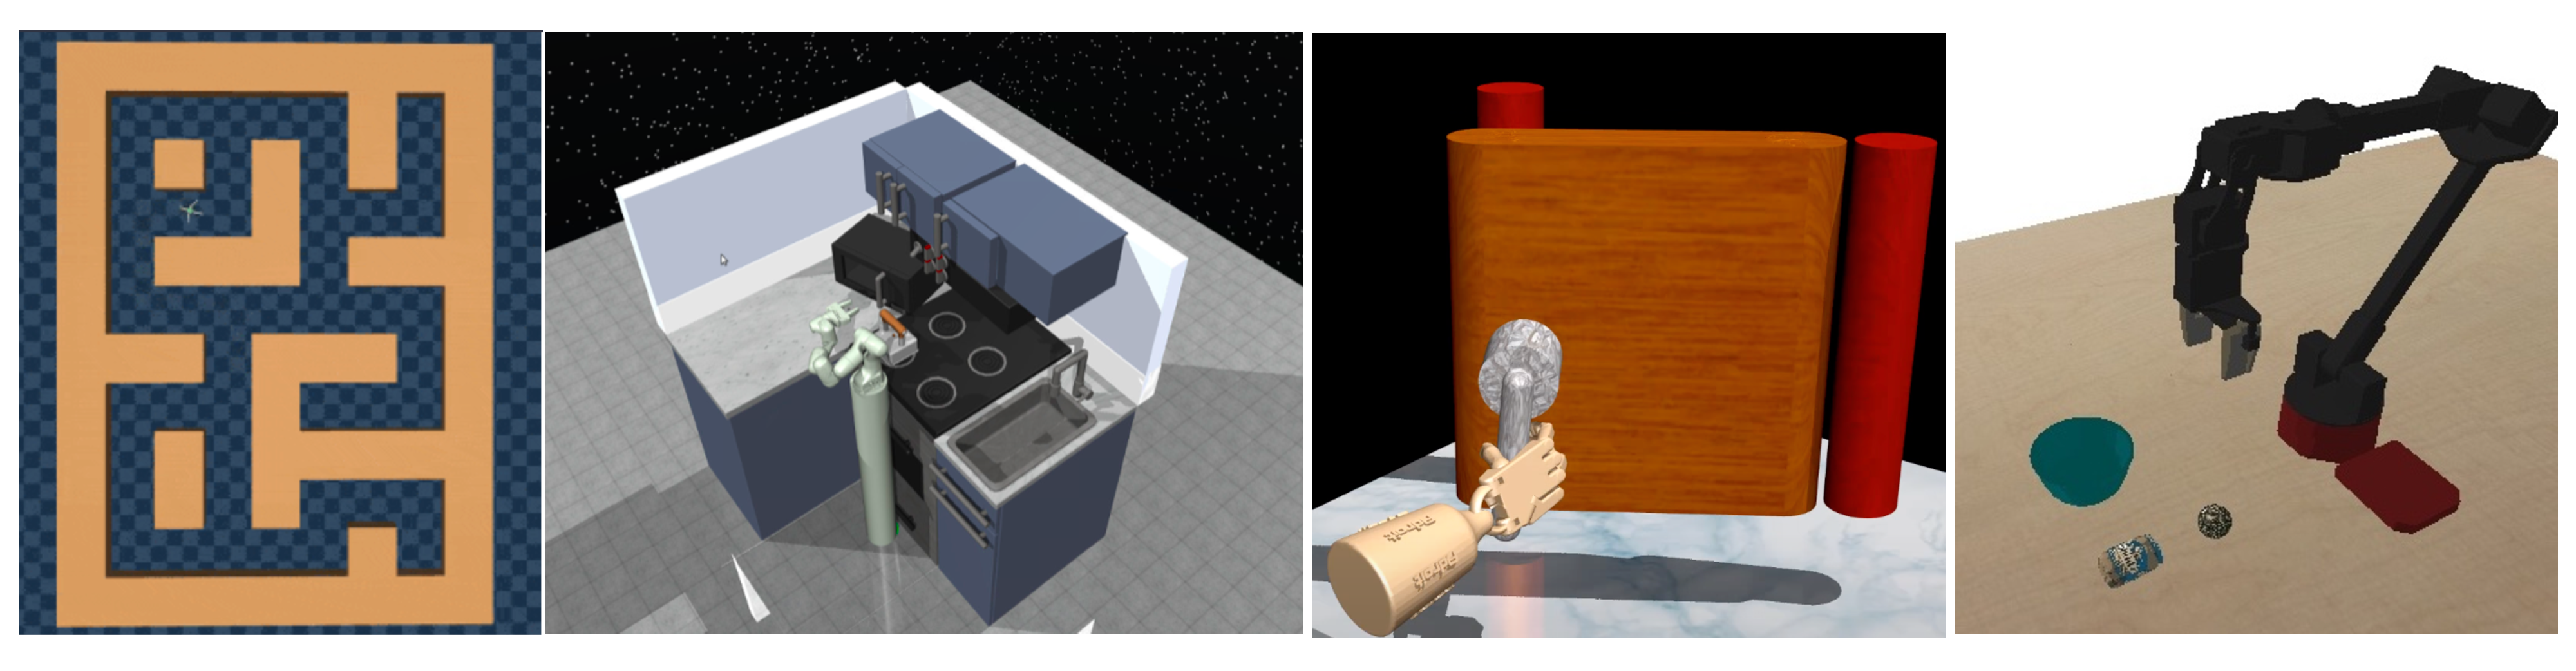
\includegraphics[width=0.99\linewidth]{chapters/cal_ql/figs-sample/envs_final.pdf}
\vspace{-0.45cm}
\caption{
\footnotesize{\textbf{Tasks:} We evaluate \methodname\ on a diverse set of benchmarks: \texttt{AntMaze} \& \texttt{Frankakitchen} domains from \cite{fu2020d4rl}, \texttt{Adroit} tasks from \cite{nair2020accelerating} and a vision-based robotic manipulation task from \cite{kumar2022pre}.}}
\label{fig:envs}
\vspace{-0.6cm}
\end{wrapfigure}
%%AK.5.6: Do we need this figure to be in the main paper given that we are tight on space?
\niparagraph{\textbf{Offline RL tasks and datasets.}} We evaluate \methodname\ on a number of benchmark tasks and datasets used by prior works~\cite{kostrikov2021offlineb,nair2020accelerating} to evaluate fine-tuning performance: \textbf{(1)} The {\texttt{AntMaze}} tasks from D4RL~\cite{fu2020d4rl} that require controlling an ant quadruped robot to navigate from a starting point to a desired goal location in a maze. The reward is +1 if the agent reaches within a pre-specified small radius around the goal and 0 otherwise. 
% We consider two kinds of maze layouts (medium and large mazes from \cite{fu2020d4rl}) and two data compositions: \textbf{play} and \textbf{diverse} that vary in coverage of actions at different regions of the state space and sub-optimality of the behavior policy. 
\textbf{(2)} The \texttt{FrankaKitchen} tasks from D4RL require controlling a 9-DoF Franka robot to attain a desired configuration of a kitchen. To succeed, a policy 
must complete four sub-tasks in the kitchen within a single rollout, and it receives a binary reward of +1/0 for every sub-task it completes. \textbf{(3)} Three \texttt{Adroit} dexterous manipulation tasks~\cite{rajeswaran2018dapg,kostrikov2021offlineb,nair2020accelerating} that require learning complex manipulation skills on a 28-DoF five-fingered hand to \textbf{(a)} manipulate a pen in-hand to a desired configuration (\texttt{pen-binary}), \textbf{(b)} open a door by unlatching the handle (\texttt{door-binary}), and \textbf{(c)} relocating a ball to a desired location (\texttt{relocate-binary}). The agent obtains a sparse binary +1/0 reward if it succeeds in solving the task. Each of these tasks only provides a narrow offline dataset consisting of 25 demonstrations collected via human teleoperation and additional trajectories collected by a BC policy.
Finally, to evaluate the efficacy of \methodname\ on a task where we learn from raw visual observations, we study \textbf{(4)} a pick-and-place task from prior work~\cite{singh2020cog,kumar2022pre} that requires learning to pick a ball and place it in a bowl, in the presence of distractors.


\iffalse

\textbf{Offline RL tasks and datasets.} We evaluate \methodname\ on a number of benchmark tasks and datasets used by prior works~\cite{kostrikov2021offlineb,nair2020accelerating} to evaluate fine-tuning performance: \textbf{(1)} The {\texttt{AntMaze}} tasks from D4RL~\cite{fu2020d4rl} that require controlling an 8-DoF ant quadruped robot to navigate from a starting point to a desired goal location in a maze. The reward is +1 if the agent reaches within a pre-specified small radius around the goal and 0 otherwise. We consider two kinds of maze layouts (medium and large mazes from \cite{fu2020d4rl}) and two data compositions: \textbf{play} and \textbf{diverse} that vary in coverage of actions at different regions of the state space and sub-optimality of the behavior policy. \textbf{(2)} The \texttt{FrankaKitchen} tasks from D4RL require controlling a 9-DoF Franka robot to attain a desired configuration of a kitchen. To succeed, a policy 
must complete four sub-tasks in the kitchen within a single rollout, and it receives a binary reward of +1/0 for every sub-task it completes. \textbf{(3)} Three \texttt{Adroit} dexterous manipulation tasks~\cite{rajeswaran2018dapg,kostrikov2021offlineb,nair2020accelerating} that require learning complex manipulation skills on a 28-DoF five-fingered hand to \textbf{(a)} manipulate a pen in-hand to a desired configuration (\texttt{pen-binary}), \textbf{(b)} open a door by unlatching the handle (\texttt{door-binary}), and \textbf{(c)} relocating a ball to a desired location (\texttt{relocate-binary}). An agent obtains a sparse binary +1/0 reward if it succeeds in solving the task. Each of these tasks only provides an extremely narrow offline dataset consisting of 25 demonstrations collected via human teleoperation and additional trajectories collected by a BC policy.
Finally, to evaluate the efficacy of \methodname\ on more challenging tasks where we must learn from raw visual observations, we study \textbf{(4)} a pick-and-place task from prior work~\cite{singh2020cog,kumar2022pre} that requires learning to pick a ball and place it in a bowl, in the presence of distractors.

\fi

\begin{figure}[t]
\begin{center}    
{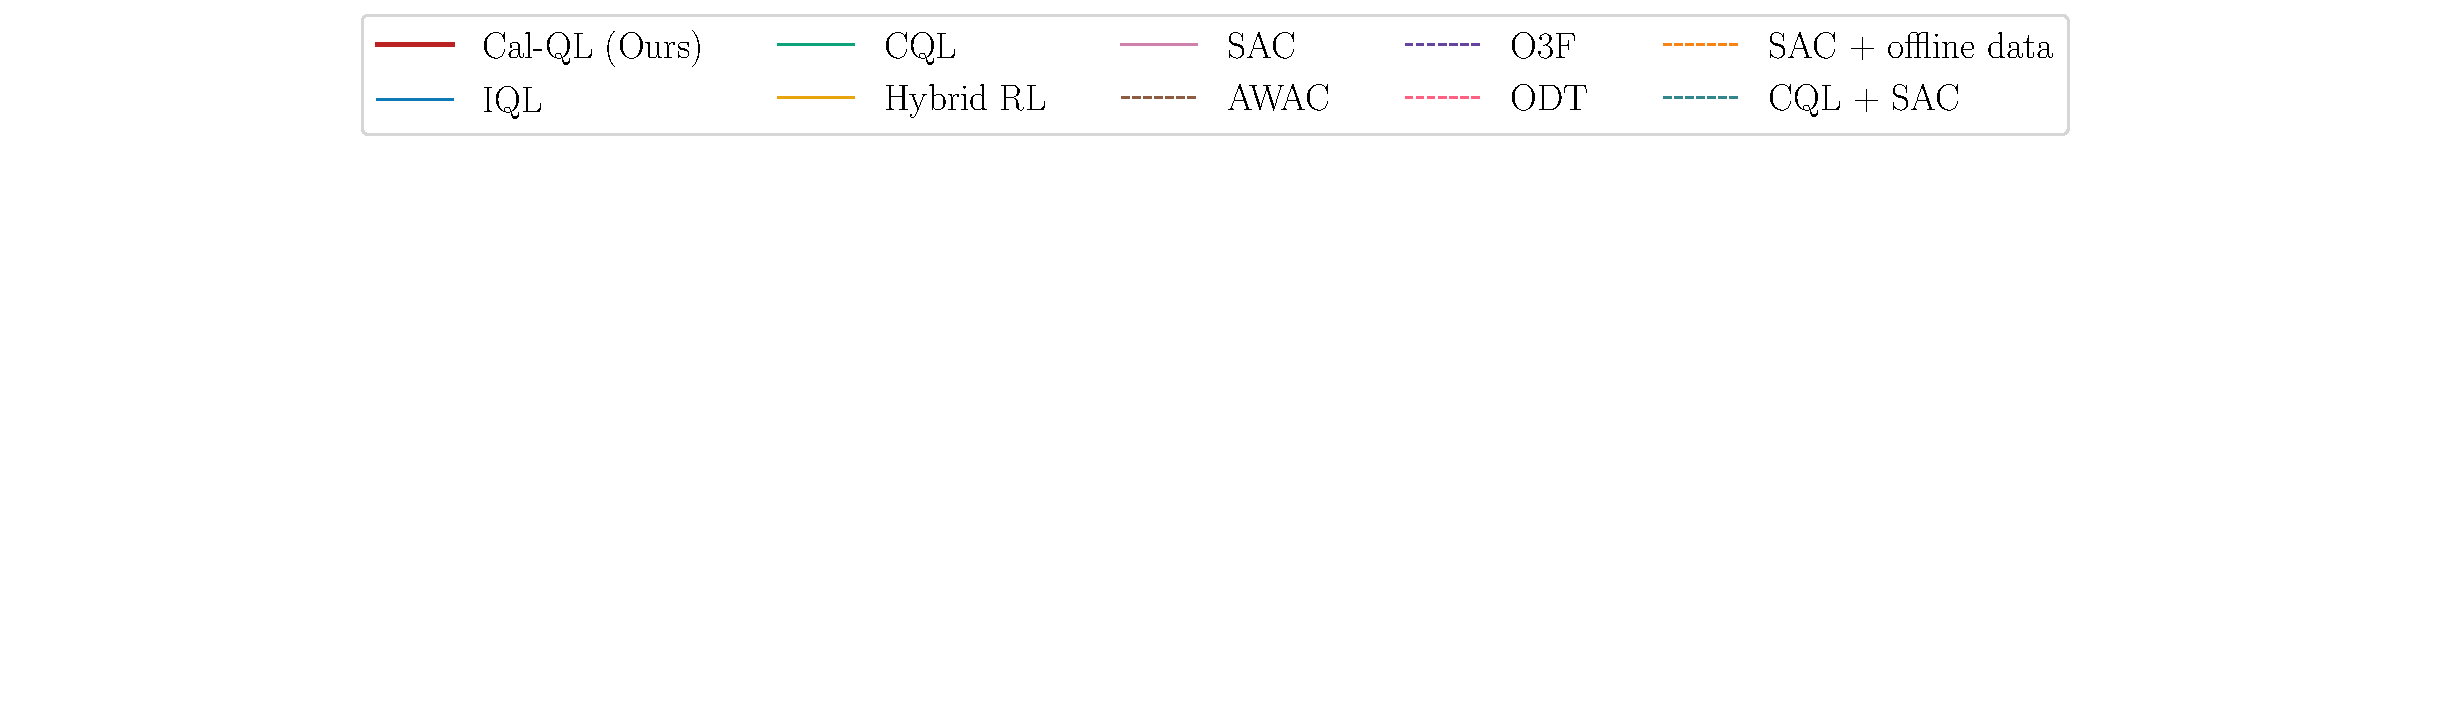
\includegraphics[clip,width=1\linewidth]{chapters/cal_ql/figs-sample/antmaze-final-caption.pdf}} 
{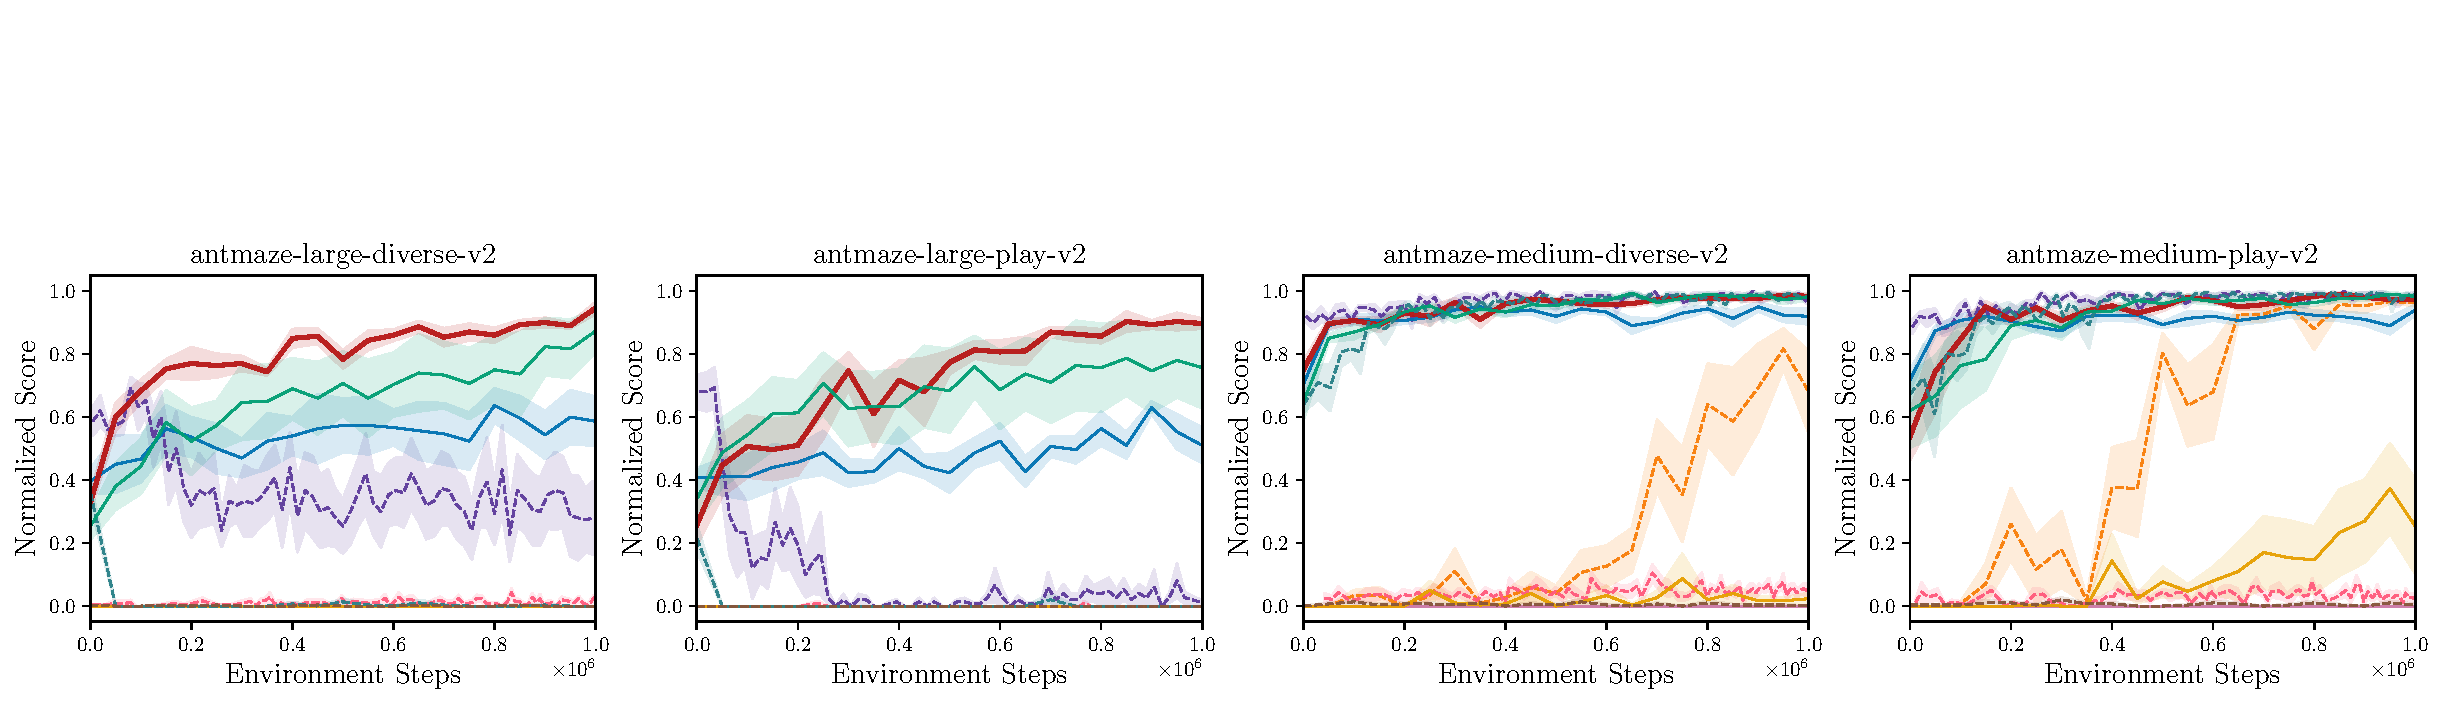
\includegraphics[clip,width=1\linewidth]{chapters/cal_ql/figs-sample/antmaze-final-plots-only.pdf}}\\{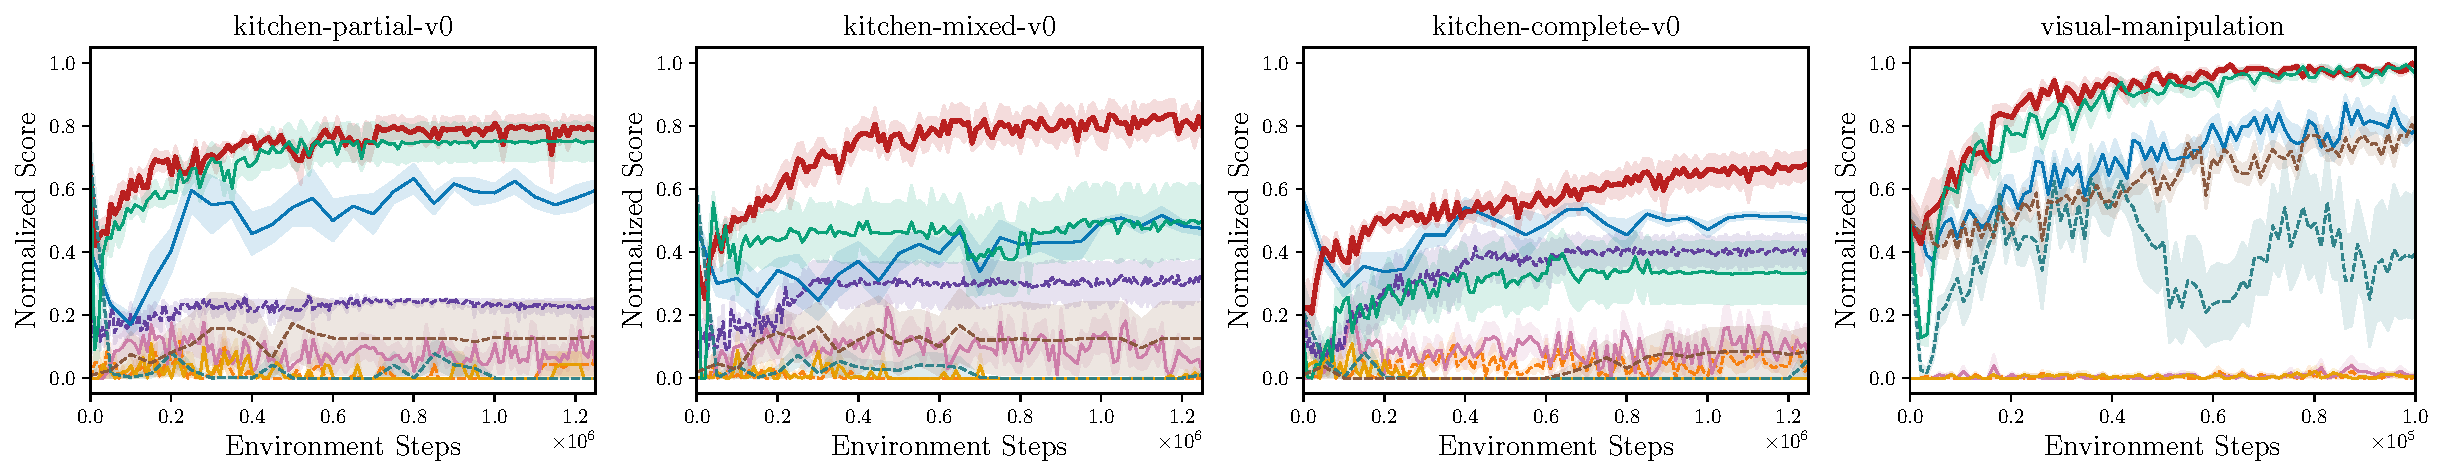
\includegraphics[clip,width=1\linewidth]{chapters/cal_ql/figs-sample/kitchen-cog-final.pdf}} {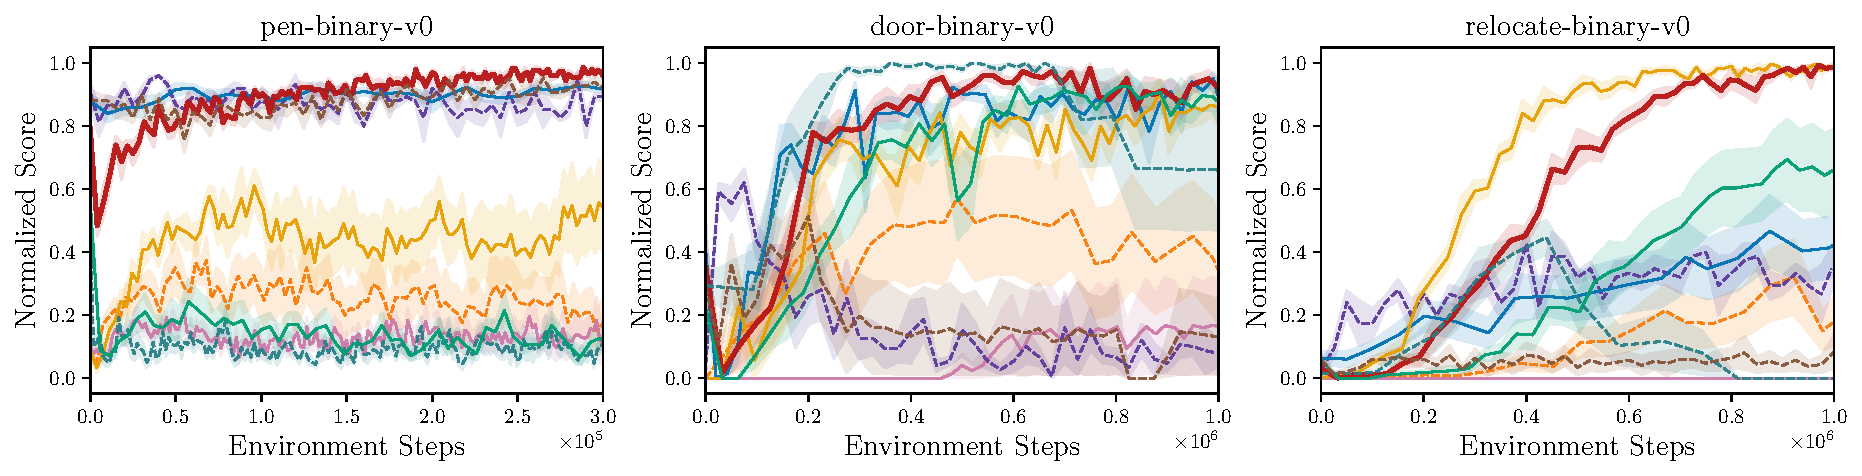
\includegraphics[clip,width=0.75\linewidth]{chapters/cal_ql/figs-sample/adroit-final.pdf}}
\end{center}
\vspace{-0.45cm}
\caption{\label{fig:all_tasks} \footnotesize{\textbf{Online fine-tuning after offline initialization on the benchmark tasks}. The plots show the online fine-tuning phase \emph{after} pre-training for each method (except SAC-based approaches which are not pre-trained). Observe that \methodname\ consistently matches or exceeds the speed and final performance of the best prior method and is the only algorithm to do so across all tasks. (6 seeds)}}
\vspace{-0.5cm}
\end{figure}

~

\noindent \textbf{Comparisons, prior methods, and evaluation protocol.} We compare \methodname\ to running online SAC~\cite{haarnoja2018soft} from scratch, as well as prior approaches that leverage offline data. This includes na\"ively fine-tuning offline RL methods such as CQL~\cite{kumar2020conservative} and IQL~\cite{kostrikov2021offlineb}, as well as fine-tuning with AWAC~\citep{nair2020accelerating}, O3F~\cite{mark2022fine} and online decision transformer (ODT)~\citep{zheng2022online}, methods specifically designed for offline RL followed by online fine-tuning. In addition, we also compare to a baseline that trains SAC~\cite{haarnoja2018soft} using both online data and offline data (denoted by ``SAC + offline data'') that mimics DDPGfD~\citep{vecerik2017leveraging} but utilizes SAC instead of DDPG. We also compare to Hybrid RL~\citep{song2023hybrid}, a recently proposed method that improves the sample efficiency of the ``SAC + offline data'' approach, and ``CQL+SAC'', which first pre-train with CQL and then run fine-tuning with SAC on a mixture of offline and online data without conservatism. More details of each method can be found in Appendix~\ref{app:hyperparam}.
We present learning curves for online fine-tuning and also quantitatively evaluate each method on its ability to improve the initialization learned from offline data measured in terms of \textbf{(i)} final performance after a pre-defined number of steps per domain and \textbf{(ii)} the cumulative regret over the course of online fine-tuning. In Section~\ref{subsec:highutd}, we run \methodname\ with a higher update-to-data (UTD) ratio and compare it to RLPD~\cite{rlpd}, a more sample-efficient version of ``SAC + offline data''.

\vspace{-0.2cm}
\subsection{Empirical Results} 
\vspace{-0.2cm}

We first present a comparison of \methodname\ in terms of the normalized performance before and after fine-tuning in Table~\ref{tab:performance} and the cumulative regret in a fixed number of online steps in Table~\ref{tab:results_regret}. Following the protocol of \cite{fu2020d4rl}, we normalize the average return values for each domain with respect to the highest possible return (+4 in FrankaKitchen; +1 in other tasks; see Appendix~\ref{appendix:normalized_score} for more details).  

\textbf{\methodname\ improves the offline initialization significantly.} Observe in Table~\ref{tab:performance} and Figure~\ref{fig:all_tasks} that while the performance of offline initialization acquired by \methodname\ is comparable to that of other methods such as CQL and IQL, \methodname\ is able to improve over its offline initialization the most by \textbf{106.9\%} in aggregate and achieve the best fine-tuned performance in \textbf{9 out of 11} tasks.

\textbf{\methodname\ enables fast fine-tuning.} 
% To understand the efficacy of \methodname\ in enabling learning quickly during online fine-tuning, we measure the cumulative regret accumulated over the course of fine-tuning. 
Observe in Table~\ref{tab:results_regret} that \methodname\ achieves the smallest regret on \textbf{8 out of 11} tasks, attaining an average regret of 0.22 which improves over the next best method (IQL) by \textbf{42\%}. Intuitively, this means that \methodname\ does not require running highly sub-optimal policies. In tasks such as \texttt{relocate-binary}, \methodname\ enjoys the fast online learning benefits associated with na\"ive online RL methods that incorporate the offline data in the replay buffer (SAC + offline data and \methodname\ are the only two methods to  attain a score of $\geq$ 90\% on this task) unlike prior offline RL methods. As shown in Figure~\ref{fig:all_tasks}, in the \texttt{kitchen} and \texttt{antmaze} domains, \methodname\ brings the benefits of fast online learning together with a good offline initialization, improving drastically on the regret metric. Finally, observe that the initial unlearning at the beginning of fine-tuning with conservative methods observed in Section~\ref{sec:empirical_analysis} is greatly alleviated in all tasks (see Appendix~\ref{app:cql_dip_zoom_in} for details).


\begin{table*}[h]
\scriptsize{
\begin{center}

\vspace{-0.1cm}
\!\!\!\!\resizebox{1.0\textwidth}{!}{
\begin{tabular}{l|c|c|c|c|c|c|c|c|c||c}
Task & CQL & IQL & AWAC & O3F & ODT & CQL+SAC & Hybrid SRL & SAC+od & SAC & Cal-QL (Ours) \\ \hline \hline
\texttt{large-diverse}  & 25 $\rightarrow$ 87 & 40 $\rightarrow$ 59 & 00 $\rightarrow$ 00 & 59 $\rightarrow$ 28 & 00 $\rightarrow$ 01 & 36 $\rightarrow$ 00 &  $\rightarrow$ 00 &  $\rightarrow$ 00 &  $\rightarrow$ 00 & 33 $\rightarrow$  \textbf{95} \\
\texttt{large-play}  & 34 $\rightarrow$ 76 & 41 $\rightarrow$ 51 & 00 $\rightarrow$ 00 & 68 $\rightarrow$ 01 & 00 $\rightarrow$ 00 & 21 $\rightarrow$ 00 &  $\rightarrow$ 00 &  $\rightarrow$ 00 &  $\rightarrow$ 00 & 26 $\rightarrow$  \textbf{90} \\
\texttt{medium-diverse}  & 65 $\rightarrow$  \textbf{98} & 70 $\rightarrow$ 92 & 00 $\rightarrow$ 00 & 92 $\rightarrow$ 97 & 00 $\rightarrow$ 03 & 64 $\rightarrow$ \textbf{98} &  $\rightarrow$ 02 &  $\rightarrow$ 68 &  $\rightarrow$ 00 & 75 $\rightarrow$ \textbf{98} \\
\texttt{medium-play}  & 62 $\rightarrow$ 98 & 72 $\rightarrow$ 94 & 00 $\rightarrow$ 00 & 89 $\rightarrow$ \textbf{99} & 00 $\rightarrow$ 05 & 67 $\rightarrow$ 98 &  $\rightarrow$ 25 &  $\rightarrow$ 96 &  $\rightarrow$ 00 & 54 $\rightarrow$ 97 \\  \hline
\texttt{partial}  & 71 $\rightarrow$ 75 & 40 $\rightarrow$ 60 & 01 $\rightarrow$ 13 & 11 $\rightarrow$ 22 & - & 71 $\rightarrow$ 00 &  $\rightarrow$ 00 &  $\rightarrow$ 07 &  $\rightarrow$ 03 & 67 $\rightarrow$ \textbf{79} \\
\texttt{mixed}  & 56 $\rightarrow$ 50 & 48 $\rightarrow$ 48 & 02 $\rightarrow$ 12 & 06 $\rightarrow$ 33 & - & 59 $\rightarrow$ 01 &   $\rightarrow$ 01 &   $\rightarrow$ 00 &   $\rightarrow$ 02 & 38 $\rightarrow$ \textbf{80} \\
\texttt{complete} & 13 $\rightarrow$ 34 & 57 $\rightarrow$ 50 & 01 $\rightarrow$ 08 & 17 $\rightarrow$ 41 & - & 21 $\rightarrow$ 06 &  $\rightarrow$ 00 & $\rightarrow$ 05 &  $\rightarrow$ 06 & 22 $\rightarrow$ \textbf{68} \\  \hline
\texttt{pen} & 55 $\rightarrow$ 13 & 88 $\rightarrow$ 92 & 88 $\rightarrow$ 92 & 91 $\rightarrow$ 89 & - & 48 $\rightarrow$ 10 &  $\rightarrow$ 54 &  $\rightarrow$ 17 &  $\rightarrow$ 11 & 79 $\rightarrow$ \textbf{99} \\
\texttt{door} & 22 $\rightarrow$ 88 & 41 $\rightarrow$ 88 & 29 $\rightarrow$ 13 & 04 $\rightarrow$ 08 & - & 29 $\rightarrow$ 66 &  $\rightarrow$ 88 &  $\rightarrow$ 39 &  $\rightarrow$ 17 & 35 $\rightarrow$ \textbf{92} \\
\texttt{relocate} & 06 $\rightarrow$ 69 & 06 $\rightarrow$ 45 & 06 $\rightarrow$ 08 & 03 $\rightarrow$ 35 & - & 01 $\rightarrow$ 00 &  $\rightarrow$ \textbf{99} &  $\rightarrow$ 16 &  $\rightarrow$ 00 & 03 $\rightarrow$ 98 \\  \hline
\texttt{manipulation} & 50 $\rightarrow$ 97 & 49 $\rightarrow$ 81 & 50 $\rightarrow$ 73 & - & - & 42 $\rightarrow$ 41 &  $\rightarrow$ 00 &  $\rightarrow$ 01 &  $\rightarrow$ 01 & 49 $\rightarrow$ \textbf{99} \\ \hline \hline
\textbf{average} & 42 $\rightarrow$ 71 & 50 $\rightarrow$ 69 & 16 $\rightarrow$ 20 & 44 $\rightarrow$ 45 & 00 $\rightarrow$ 02 & 42 $\rightarrow$ 29 &  $\rightarrow$ 24 &  $\rightarrow$ 23 &  $\rightarrow$ 04 & 44 $\rightarrow$ \textbf{90} \\ \hline
\textbf{improvement} & + 71.0\%  & + 37.7\%  & + 23.7\%  & + 3.0\%  & N/A  & - 30.3\%  & N/A &  N/A &  N/A & \textbf{+ 106.9\%}  \\
\end{tabular}}
\vspace{-0.15cm}
a\caption{\footnotesize{\textbf{Normalized score before \& after online fine-tuning.} Observe that \methodname\ improves over the best prior fine-tuning method and attains a much larger performance improvement over the course of online fine-tuning. The numbers represent the normalized score out of 100 following the convention in \citep{fu2020d4rl}.} \label{tab:performance}}

\vspace{-0.3cm}
\end{center}
}
\end{table*}

% \begin{wraptable}{r}{0.66\linewidth}
\begin{table*}[h]

\vspace{-0.4cm}
\small{
\begin{center}
\resizebox{1.0\textwidth}{!}{
\begin{tabular}{l|c|c|c|c|c|c|c|c|c||c}
Task & CQL & IQL & AWAC & O3F & ODT & CQL+SAC & Hybrid RL & SAC+od & SAC & Cal-QL (Ours)\\ \hline \hline 
\texttt{large-diverse}  & 0.35 & 0.46 & 1.00 & 0.62 & 0.98 & 0.99 & 1.00 & 1.00 & 1.00 & \textbf{0.20}  \\
\texttt{large-play}     & 0.32 & 0.52 & 1.00 & 0.91 & 1.00 & 0.99 & 1.00 & 1.00 & 1.00 & \textbf{0.28}  \\
\texttt{medium-diverse} & 0.06 & 0.08 & 0.99 & \textbf{0.03} & 0.95 & 0.06 & 0.98 & 0.77 & 1.00 & 0.05  \\
\texttt{medium-play}    & 0.09 & 0.10 & 0.99 & \textbf{0.04} & 0.96 & 0.06 & 0.90 & 0.47 & 1.00 & 0.07  \\ \hline
\texttt{partial}                   & 0.31 & 0.49 & 0.89 & 0.78 & - & 0.97 & 0.98 & 0.98 & 0.92 & \textbf{0.27}  \\
\texttt{mixed}                     & 0.55 & 0.60 & 0.88 & 0.72 & - & 0.97 & 0.99 & 1.00 & 0.91 & \textbf{0.27}  \\
\texttt{complete}                  & 0.70 & 0.53 & 0.97 & 0.66 & - & 0.99 & 0.99 & 0.96 & 0.91 & \textbf{0.44}  \\ \hline
\texttt{pen}                       & 0.86 & \textbf{0.11} & 0.12 & 0.13 & - & 0.90 & 0.56 & 0.75 & 0.87 & \textbf{0.11}  \\
\texttt{door}                      & 0.36 & 0.25 & 0.81 & 0.82 & - & \textbf{0.23} & 0.35 & 0.60 & 0.94 & \textbf{0.23}  \\
\texttt{relocate}                  & 0.71 & 0.74 & 0.95 & 0.71 & - & 0.86 & \textbf{0.30} & 0.89 & 1.00 & 0.43  \\ \hline
\texttt{manipulation}              & 0.15 & 0.32 & 0.38 & - & - & 0.61 & 1.00 & 1.00 & 0.99 & \textbf{0.11}   \\ \hline \hline
\textbf{average}              & 0.41 & 0.38 & 0.82 & 0.54 & 0.97 & 0.69 & 0.82 & 0.86 & 0.96 & \textbf{0.22} 

\end{tabular}}
\vspace{-0.05cm}
\caption{\footnotesize{\textbf{Cumulative regret averaged over the steps of fine-tuning.} The smaller the better and 1.00 is the worst. \methodname\ attains the smallest overall regret, achieving the best performance among 8 / 11 tasks.}}
\label{tab:results_regret}

\vspace{-0.6cm}
\end{center}}
% \end{wraptable}
\end{table*}

\vspace{-0.1cm}
\subsection{\methodname\ With High Update-to-Data (UTD) Ratio}
\label{subsec:highutd}
\vspace{-0.2cm}


We can further enhance the online sample efficiency of \methodname\ by increasing the number of gradient steps per environment step made by the algorithm. The number of updates per environment step is usually called the update-to-data (UTD) ratio.
% In Figure~\ref{fig:utd-cog}, we present the performance of \methodname\ with $\text{UTD}=5$ on the \texttt{visual-manipulation} task. We can see that \methodname\ can achieve higher sample efficiency by using $\text{UTD}=5$, and the initial unlearning disappears completely which we studied previously in Section~\ref{sec:empirical_analysis}. Interestingly, while prior fine-tuning methods such as IQL do not improve with a higher UTD (see Figure~\ref{fig:utd-cog}), \methodname\ and CQL benefit from using a higher UTD ratio. We will further discuss this in Appendix~\ref{appendix:more_discussion_on_finetuning}.
In standard online RL, running off-policy Q-learning with a high UTD value (e.g., 20, compared to the typical value of 1) often results in challenges pertaining to overfitting~\citep{li2023efficient, redq, rlpd, replaybarrier}. As expected, we noticed that running \methodname\ with a high UTD value also leads these overfitting challenges. To address these challenges in high UTD settings, we combine \methodname\ with the Q-function architecture in recent work, RLPD~\citep{rlpd} (i.e., we utilized layer normalization in the Q-function and ensembles akin to \citep{redq}), that attempts to tackle overfitting challenges. Note that \methodname\ still first pre-trains on the offline dataset using Equation~\ref{eqn:cal_ql_training} followed by online fine-tuning, unlike RLPD that runs online RL right from the start.
In Figure~\ref{fig:rlpd}, we compare \methodname\ ($\text{UTD}=20$) with RLPD~\cite{rlpd} ($\text{UTD}=20$) and also \methodname\ ($\text{UTD}=1$) as a baseline. Observe that \methodname\ ($\text{UTD}=20$) improves over \methodname\ ($\text{UTD}=1$) and training from scratch (RLPD).   

\iffalse
%%AK: This is the original version of this section

We can further enhance the online sample efficiency of \methodname\ by increasing the number of gradient steps per environment step made by the algorithm. The number of updates per environment step is usually called the update-to-data (UTD) ratio. We will now evaluate \methodname\ with a high UTD ratio. In Figure~\ref{fig:utd-cog}, we present the performance of \methodname\ with $\text{UTD}=5$ on the \texttt{visual-manipulation} task. We can see that \methodname\ can achieve higher sample efficiency by using $\text{UTD}=5$, and the initial unlearning disappears completely which we studied previously in Section~\ref{sec:empirical_analysis}. Interestingly, while prior fine-tuning methods such as IQL do not improve with a higher UTD (see Figure~\ref{fig:utd-cog}), \methodname\ and CQL benefit from using a higher UTD ratio. We will further discuss this in Appendix~\ref{appendix:more_discussion_on_finetuning}.

We noticed that simply running \methodname\ with an even higher UTD value (e.g., 20) leads to previously-observed challenges pertaining to overfitting~\citep{li2023efficient, redq, rlpd, replaybarrier}. To address these challenges in high UTD settings, we ran \methodname\ in conjunction with the Q-function architecture in \cite{rlpd} (i.e., we utilized layer normalization in the Q-function and ensembles akin to \cite{redq}) to prevent overfitting. Note that \methodname\ still first pre-trains on the offline dataset using Equation~\ref{eqn:cal_ql_training} followed by online fine-tuning, unlike RLPD that runs online RL from scratch on offline and online data. 
In Figure~\ref{fig:rlpd}, we compare \methodname\ ($\text{UTD}=20$) with RLPD~\cite{rlpd} ($\text{UTD}=20$) and also \methodname\ ($\text{UTD}=1$) as a baseline. Observe that \methodname\ ($\text{UTD}=20$) improves over \methodname\ ($\text{UTD}=1$) and training from scratch (RLPD).   

\begin{figure}[ht]
\vspace{-0.3cm}
\begin{center}
\centerline{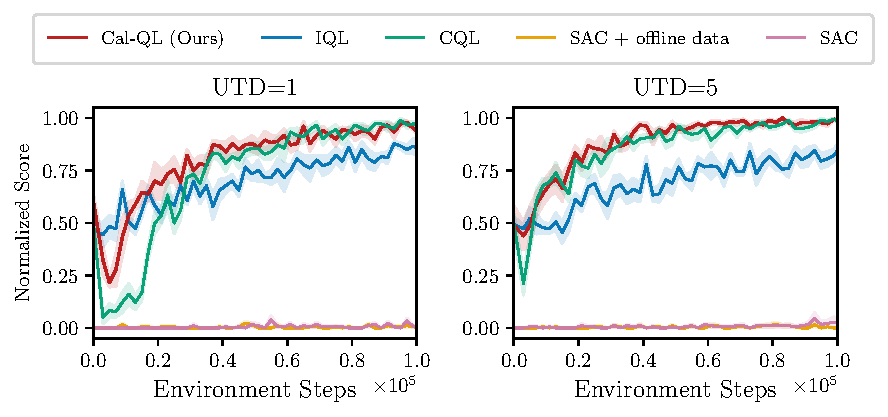
\includegraphics[width=0.55\textwidth]{chapters/cal_ql/figs-sample/cog-highutd-final.pdf}}
\vspace{-0.3cm}
\caption{\label{fig:utd-cog}\footnotesize{\textbf{UTD ablation}: We observe that using a higher UTD ratio can lead to higher sample efficiency for \methodname\ and CQL but not for IQL.}}
\end{center}
\vspace{-0.9cm}
\end{figure}

\fi

\begin{figure}[h]
\begin{center}    
{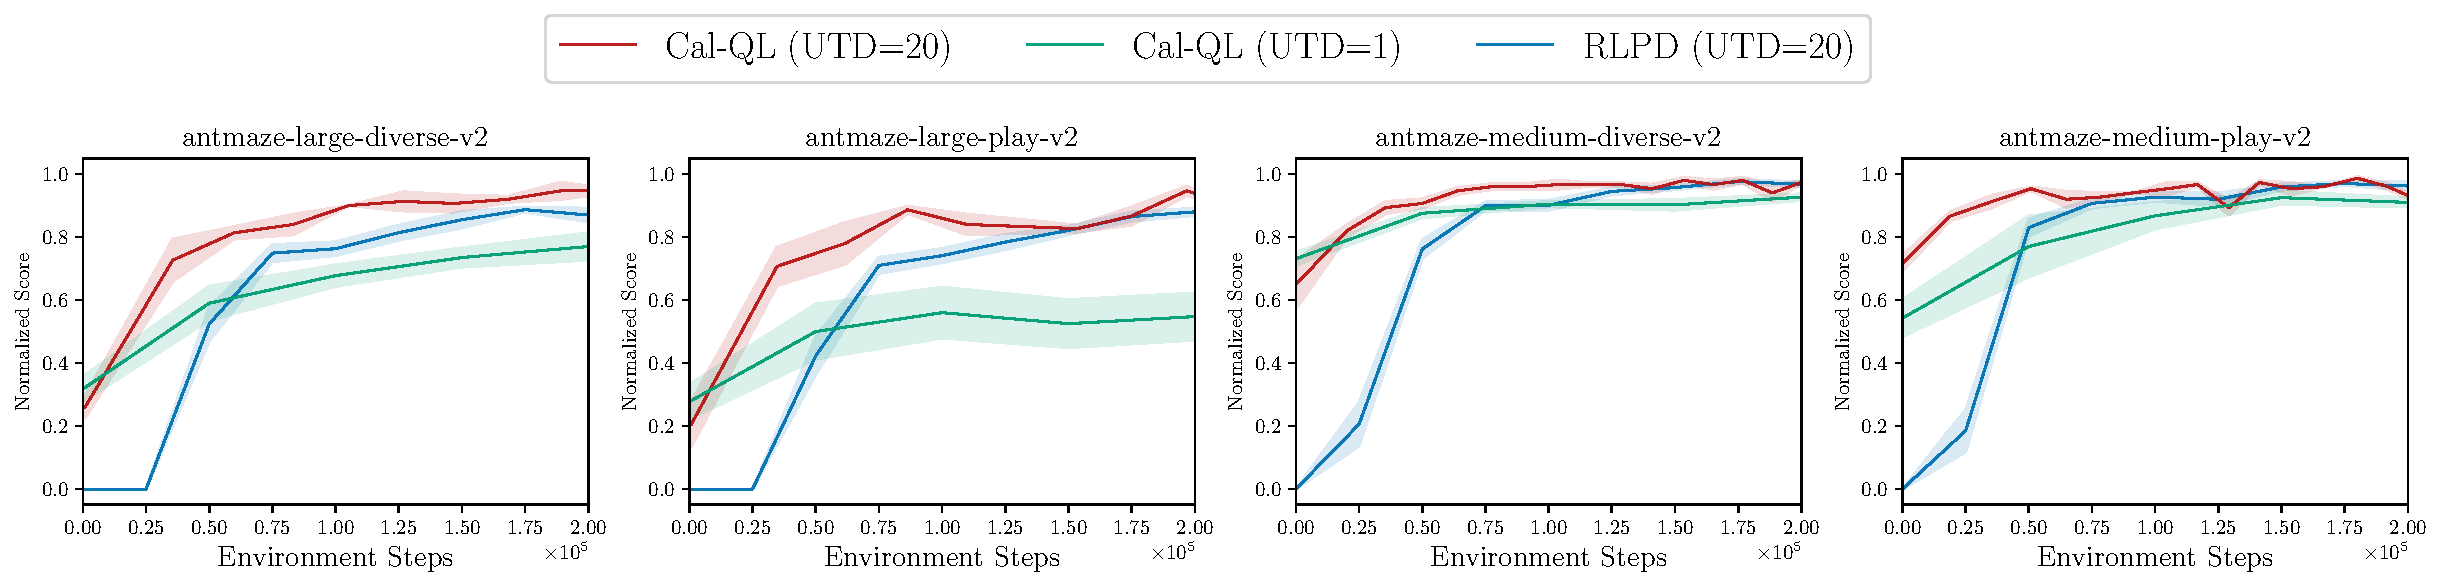
\includegraphics[clip,width=1\linewidth]{chapters/cal_ql/figs-sample/antmaze-utd20-rlpd-final.pdf}} {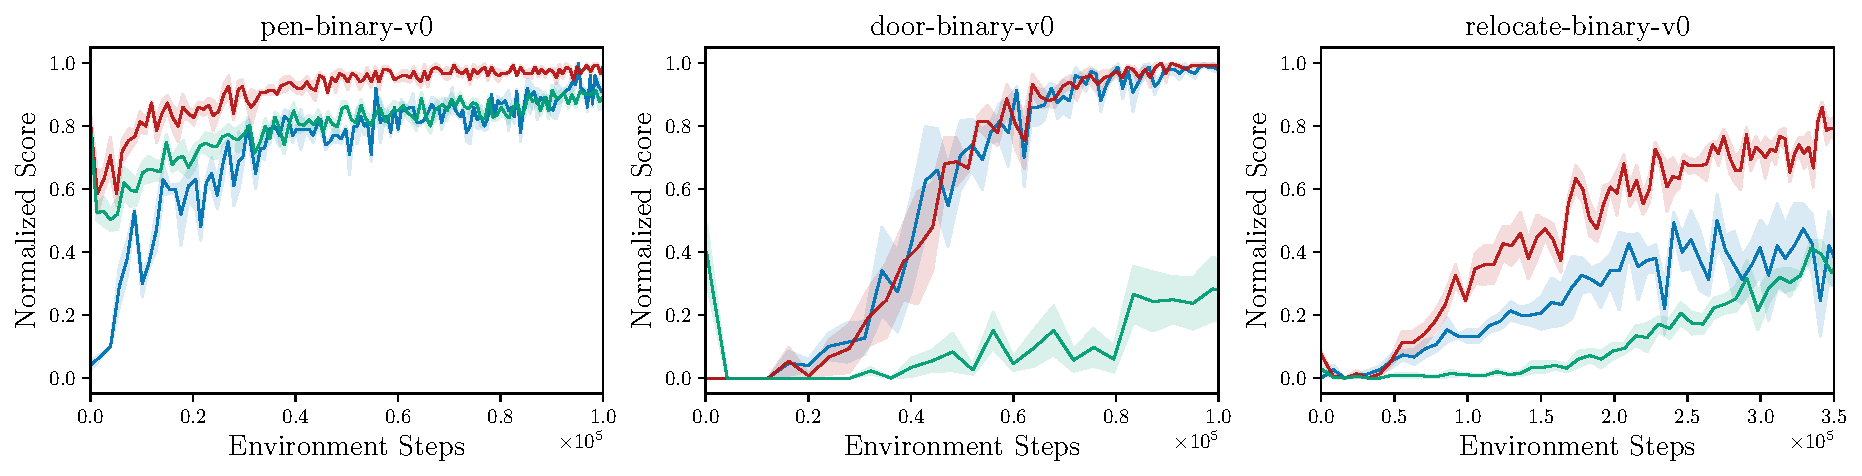
\includegraphics[clip,width=0.75\linewidth]{chapters/cal_ql/figs-sample/adroit-rlpd-final.pdf}}
\end{center}
\vspace{-0.3cm}
\caption{\label{fig:rlpd} \footnotesize{\textbf{\methodname\ with UTD=20}. Incorporating design choices from RLPD enables \methodname\ to achieve sample-efficient fine-tuning with UTD=20. Specifically, \methodname\ generally attains similar or higher asymptotic performance as RLPD, while also exhibiting a smaller cumulative regret.}}
\vspace{-0.6cm}
\end{figure}





\vspace{-0.2cm}
\subsection{Understanding the Behavior of \methodname}
\label{subsec:diagonistic}
\vspace{-0.3cm}

In this section, we aim to understand the behavior of \methodname\ by performing controlled experiments that modify the dataset composition, and by investigating various metrics to understand the properties of scenarios where utilizing \methodname\ is especially important for online fine-tuning.         

\textbf{Effect of data composition.} To understand the efficacy of \methodname\ with different data compositions, we ran it on a newly constructed fine-tuning task on the medium-size \texttt{AntMaze} domain with a low-coverage offline dataset, which is generated via a scripted controller that starts from a fixed initial position and navigates the ant to a fixed goal position. In Figure~\ref{fig:ant-narrow}, we plot the performance of \methodname\ and baseline CQL (for comparison) on this task, alongside the trend of average Q-values over the course of offline pre-training (to the left of the dashed vertical line, before 250 training epochs) and online fine-tuning (to the right of the vertical dashed line, after 250 training epochs), and the trend of \emph{bounding rate}, i.e., the fraction of transitions in the data-buffer for which the constraint in \methodname\ actively lower-bounds the learned Q-function with the reference value. For comparison, we also plot these quantities for a diverse dataset with high coverage on the task (we use the \texttt{antmaze-medium-diverse} from \cite{fu2020d4rl} as a representative diverse dataset) in Figure~\ref{fig:ant-narrow}. 

Observe that for the diverse dataset, both na\"ive CQL and \methodname\ perform similarly, and indeed, the learned Q-values behave similarly for both of these methods. In this setting, online learning doesn't spend samples to correct the Q-function when fine-tuning begins leading to a low bounding rate, almost always close to 0. Instead, with the narrow dataset, we observe that the Q-values learned by na\"ive CQL are much smaller, and are corrected once fine-tuning begins. This correction co-occurs with a drop in performance (solid blue line on left), and na\"ive CQL is unable to recover from this drop. \methodname\, which calibrates the scale of the Q-function for many more samples in the dataset, stably transitions to online fine-tuning with no unlearning (solid red line on left). 

\begin{wrapfigure}{r}{0.54\textwidth}
\vspace{-0.35cm}
\centering
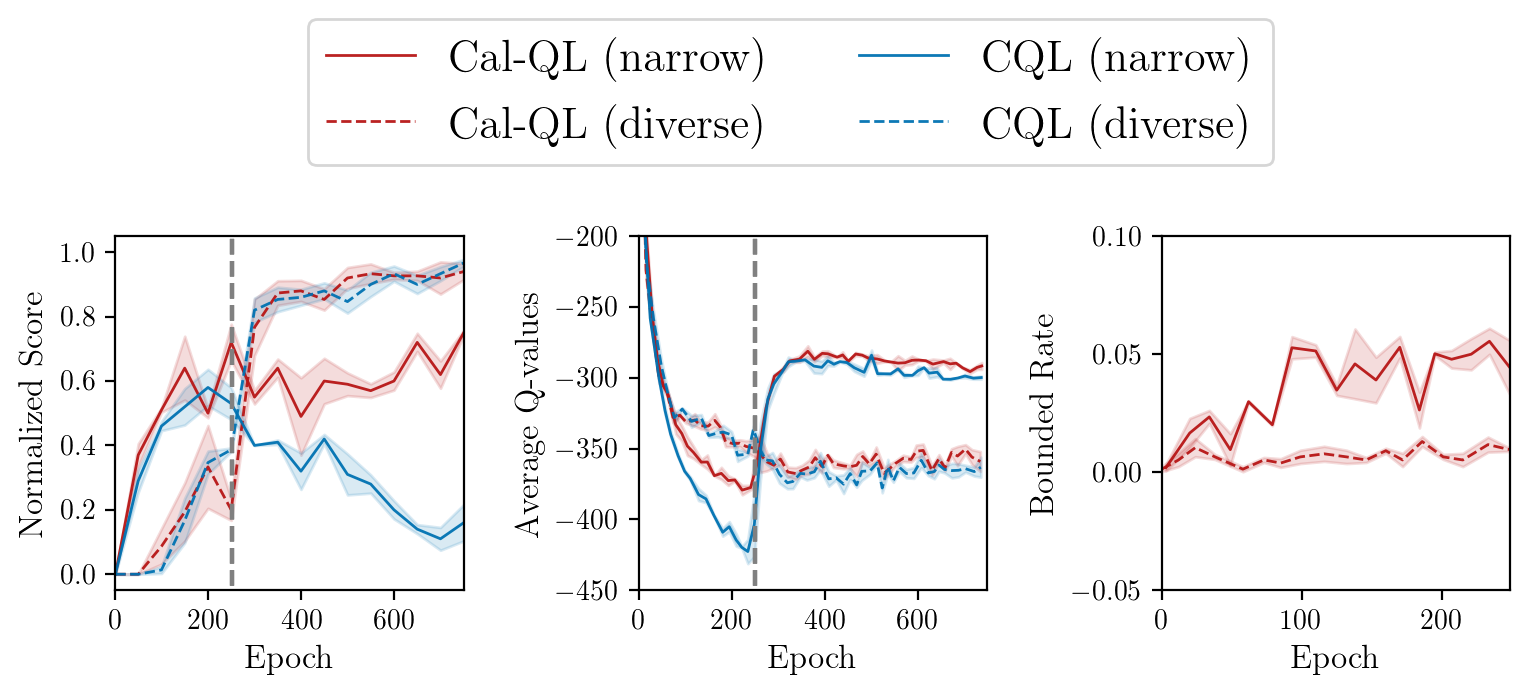
\includegraphics[width=0.97\linewidth]{chapters/cal_ql/figs-sample/diagnose-1.png}
\vspace{-0.3cm}
\caption{
\footnotesize{\textbf{Performance of \methodname\ with data compositions.} \methodname\ is most effective with narrow datasets, where Q-values need to be corrected at the beginning of fine-tuning.}
}
\label{fig:ant-narrow}
\vspace{-0.35cm}
\end{wrapfigure}


This suggests that in settings with narrow datasets (e.g., in the experiment above and in the \texttt{adroit} and \texttt{visual-manipulation} domains from Figure~\ref{fig:all_tasks}), Q-values learned by na\"ive conservative methods are more likely to be smaller than the ground-truth Q-function of the behavior policy due to function approximation errors. Hence utilizing \methodname\ to calibrate the Q-function against the behavior policy can be significantly helpful. On the other hand, with significantly high-coverage datasets, especially in problems where the behavior policy is also random and sub-optimal, Q-values learned by na\"ive methods are likely to already be calibrated with respect to those of the behavior policy. Therefore no explicit calibration might be needed (and indeed, the bounding rate tends to be very close to 0 as shown in Figure~\ref{fig:ant-narrow}). In this case, \methodname\ will revert back to standard CQL, as we observe in the case of the diverse dataset above. This intuition is also reflected in Theorem~\ref{thm:main-thm-informal}: when the reference policy $\mu$ is close to a narrow, expert policy, we would expect \methodname\ to be especially effective in controlling the efficiency of online fine-tuning. \textbf{We also present a diagnostic study of \methodname\ when the reference value function is estimated by fitting a neural network in Appendix~\ref{app:nn_value_function}}, and find that estimation errors in this model of the reference function do not affect performance significantly. 




\vspace{-0.2cm}
\vspace{-0.2cm}
\section{Discussion and Limitations}
\vspace{-0.2cm}

In this chapter, we developed \methodname\, a method for acquiring conservative offline initializations that facilitate fast online fine-tuning. \methodname\ learns conservative value functions that are constrained to be larger than the value function of a reference policy. This form of calibration allows us to avoid initial unlearning when fine-tuning with conservative methods, while also retaining the effective asymptotic performance that these methods exhibit. Our theoretical and experimental results highlight the benefit of \methodname\ in enabling fast online fine-tuning. 
% Specifically, \methodname\ improves over a number of prior approaches on 9/11 tasks that we study. 
While \methodname\ outperforms prior methods, we believe that we can develop even more effective methods by adjusting calibration and conservatism more carefully. A limitation of our work is that we do not consider fine-tuning setups where pre-training and fine-tuning tasks are different, but this is an interesting avenue for future work. Theoretically, our analysis can be improved via a more precise treatment of pessimism, and this is an avenue for future work.

\end{document}
